\title{Note on error analysis of the extracted time resolution using the automated 6-bar analysis program}
\date{January 18, 2015}

\documentclass[12pt]{article}

\usepackage{hyperref}
\usepackage{cite}

\usepackage{graphicx}
\usepackage{epsfig}
\usepackage{epstopdf}

\usepackage[pdf]{pstricks}

\usepackage{mathtools}
\newcommand{\defeq}{\vcentcolon=}

\usepackage{float}
\restylefloat{table}

%! To create a place-holder figure
\newcommand{\dummyfig}[1]{
  \centering
  \fbox{
    \begin{minipage}[c][0.33\textheight][c]{0.5\textwidth}
      \centering{#1}
    \end{minipage}
  }
}

\begin{document}
\maketitle

% \begin{abstract}
% This is the paper's abstract \ldots
% \end{abstract}

 
\begin{enumerate}
	\item This analysis is restricted to the analysis of the T histograms and their fits only. A full analysis should include a study of the fits to the 2D and 1D TW histograms.
		\begin{enumerate}
			\item In my study I have used a bin width of 0.25 TDC counts; I see that some bars have been analysed with a bin width of 0.25 TDC counts and then others with a bin width of 1 TDC counts. The latter produces a bias in estimating the standard deviation of the T distribution of the smaller bars. The official results for these particular bars did not suffer from this bias for in those cases a bin width of 0.25 TDC counts was used.
		\end{enumerate}
	\item Only fits to res\_2\_3\_4\_pointXX\_cont are considered and that too in the Normal Order.
\end{enumerate}

\section{Introduction}

% The time resolution of the FTOF system shown in Figure 5(b) was extracted using the automated analysis program developed at USC (Section 12.2). As per the optimal binning requirements, the analysis program needs to be able to analyze up to 135 data points (for the longest counters). The stability of the program depends on the stability of numerous statistical fits performed at each point, which in turn depends on the statistics at each point. Even after four days of data taking per 6-bar set, sometimes the statistics are not enough to run a \"fully constrained\" statistical fit and some of the restrictions need to be \"eased off\".  For example, the standard $\chi^{2}$ fit will \"often fail\" and ROOT fit option \"WW\" needs to be used to guarantee stability of the program over all 135 data points. This leads to certain systematic effects in the extraction of the time resolution. The point of this note is to demonstrate that effects of such systematics on the extracted time resolution is minimal and any variations finally seen, for example in Figure 5(b) is due to the variation in the quality of the scintillar bars.

Even after 4 days of data taking, the statistics are low in that standard deviation estimated from fits to the T histogram are biased and do not approach that asymptotic stable value. This is shown by way of plots that compares the fitted (using ROOT implemented Maximum Likelihood(MLE) and the standard Chi-Square statistic(CSQ)) $\mu$ and $\sigma$ to the simulated $\mu_{T}$ and $\sigma_{T}$ for various N values. The $\sigma_{T}$ simulated reflects the range of standard deviation of the T-histograms. The N values for the FTOF T-histograms is between 100 and 600.

\begin{figure*}[ht]
	%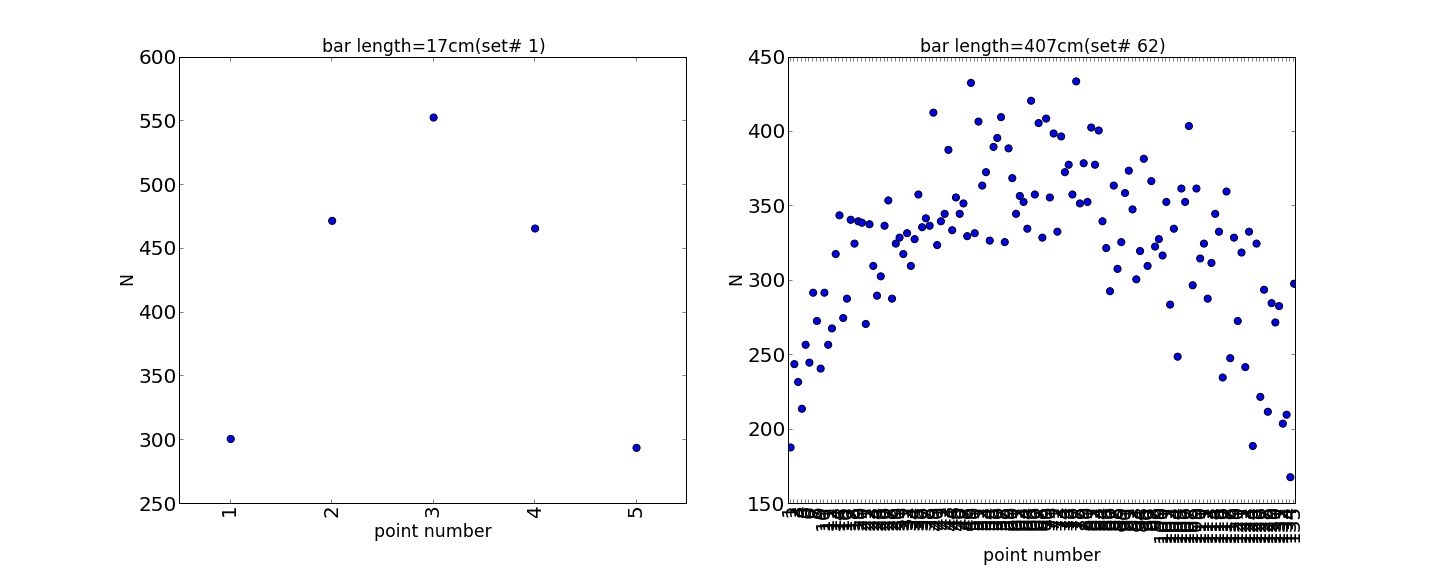
\includegraphics[height=2in,width=5in]{bar_stats_write-up_N-vs-p.png}
	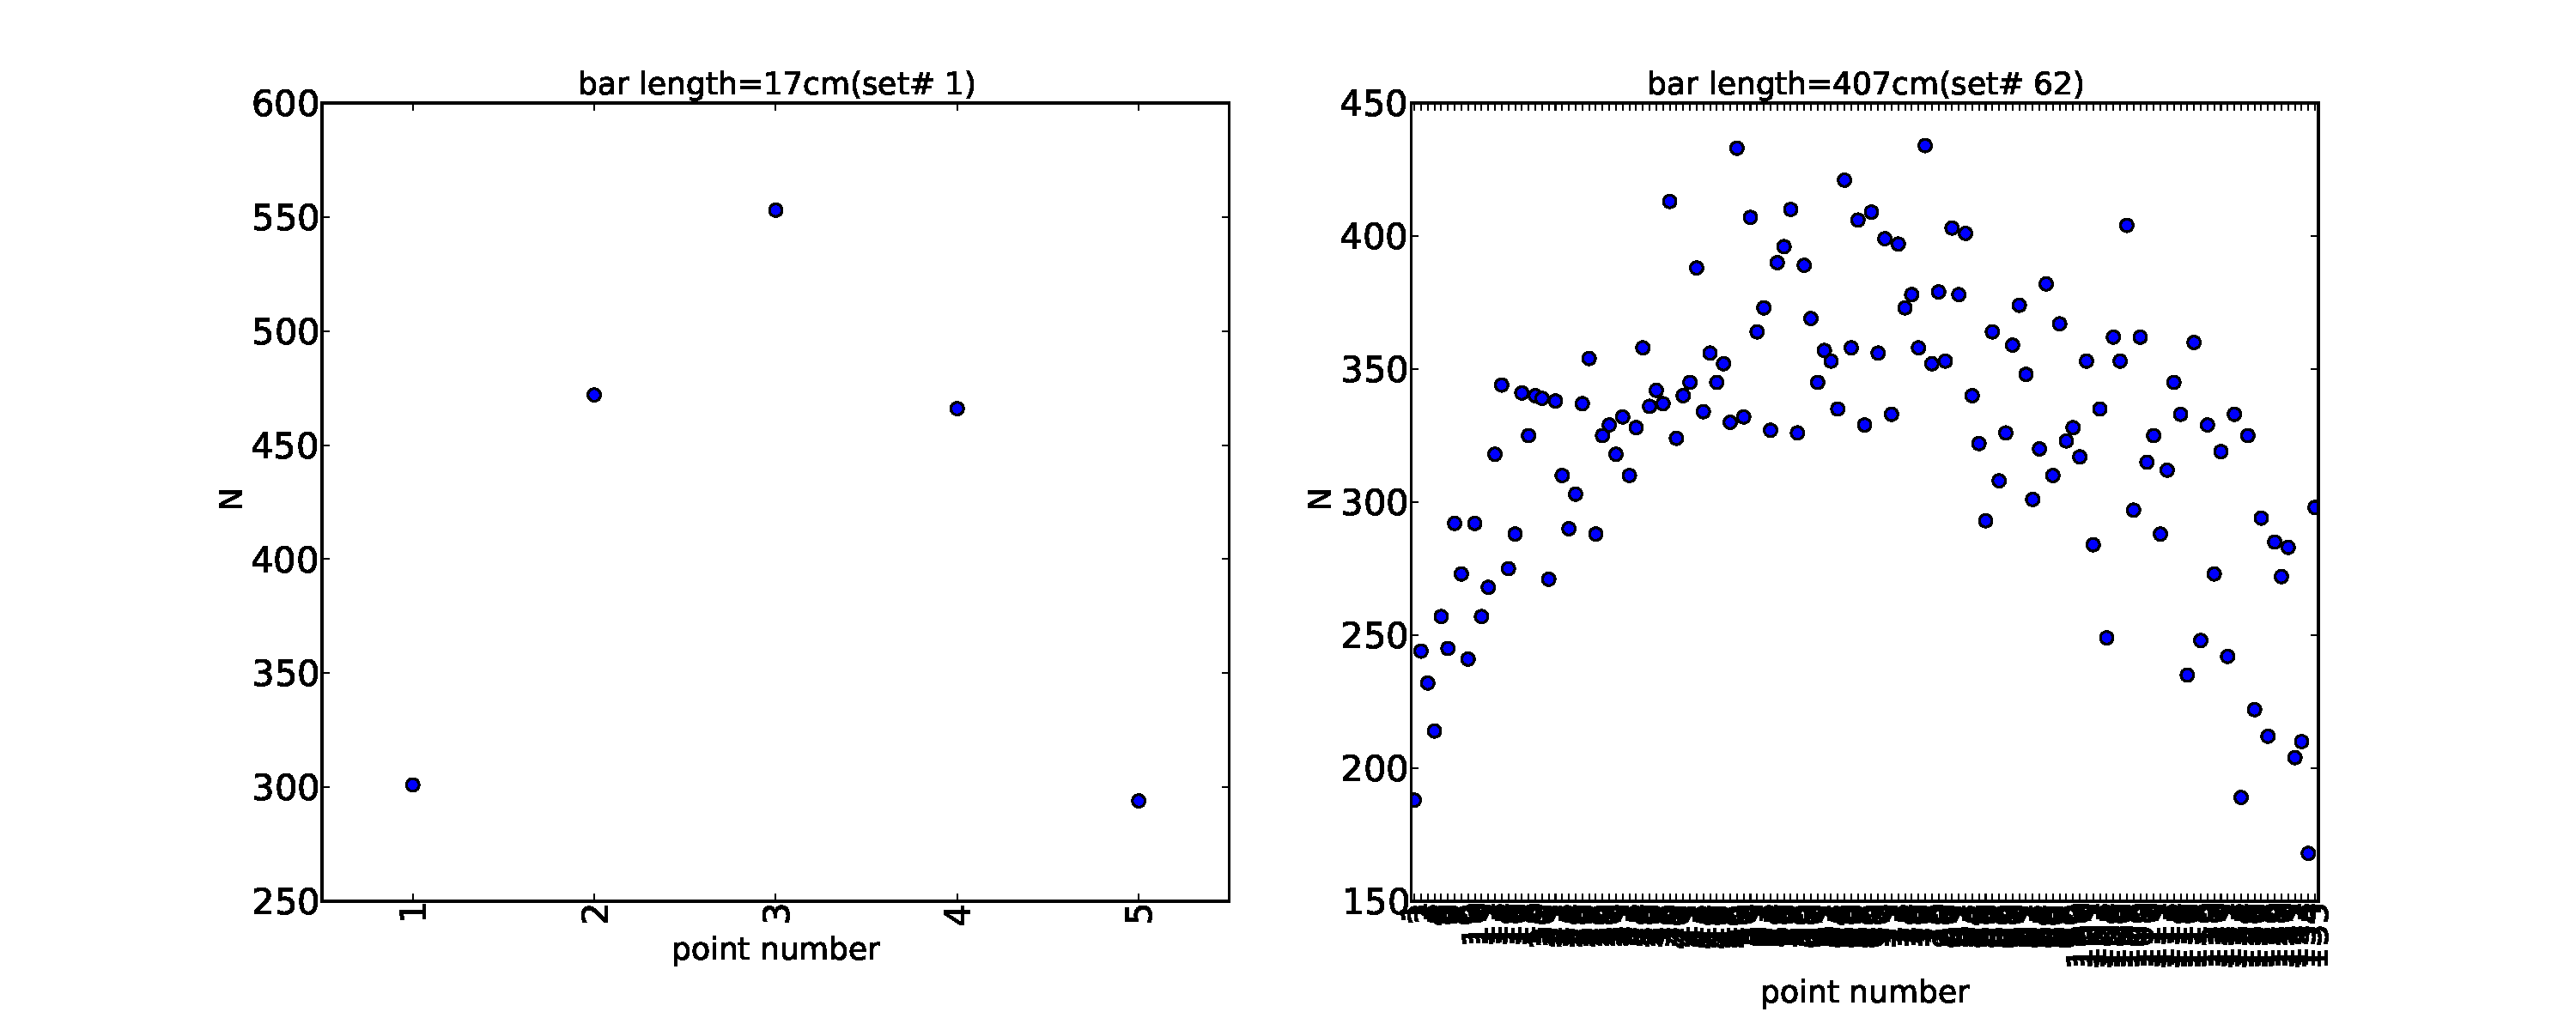
\includegraphics[height=2in,width=5in]{bar_stats_write-up_N-vs-p.pdf}
	\caption{N vs. P for the shortest and longest counters}
	\label{fig1}
\end{figure*}

%\clearpage

\begin{figure*}[ht]
	%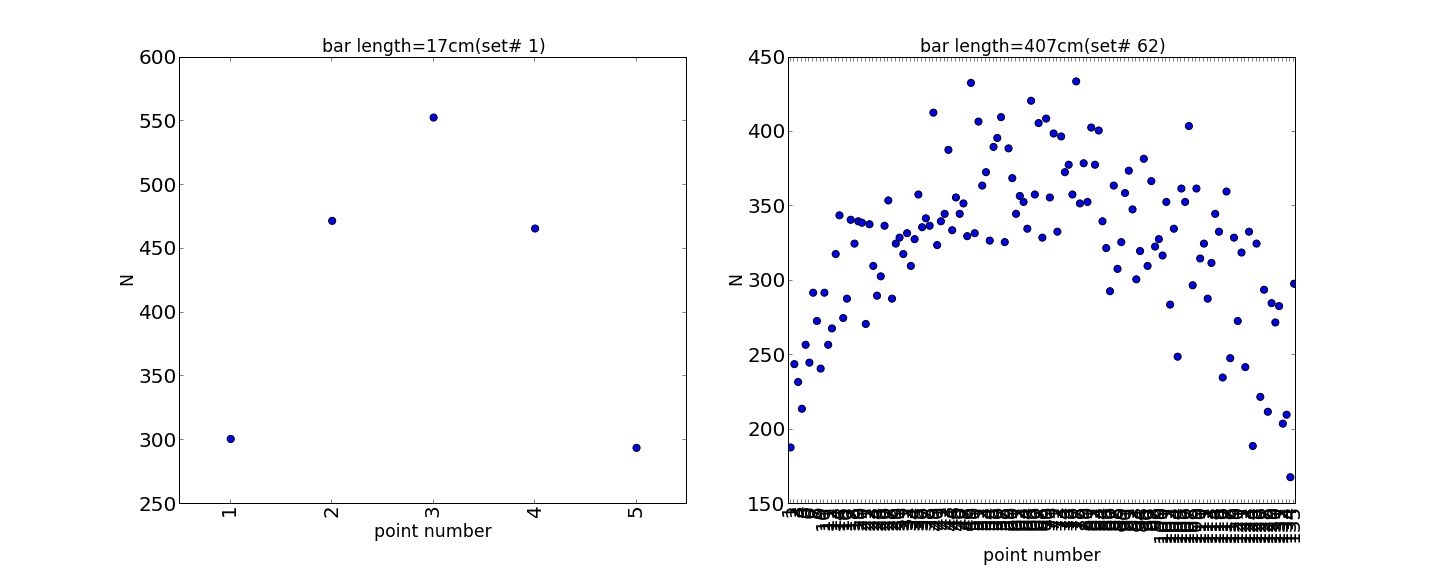
\includegraphics[height=2in,width=5in]{bar_stats_write-up_N-vs-p.png}
	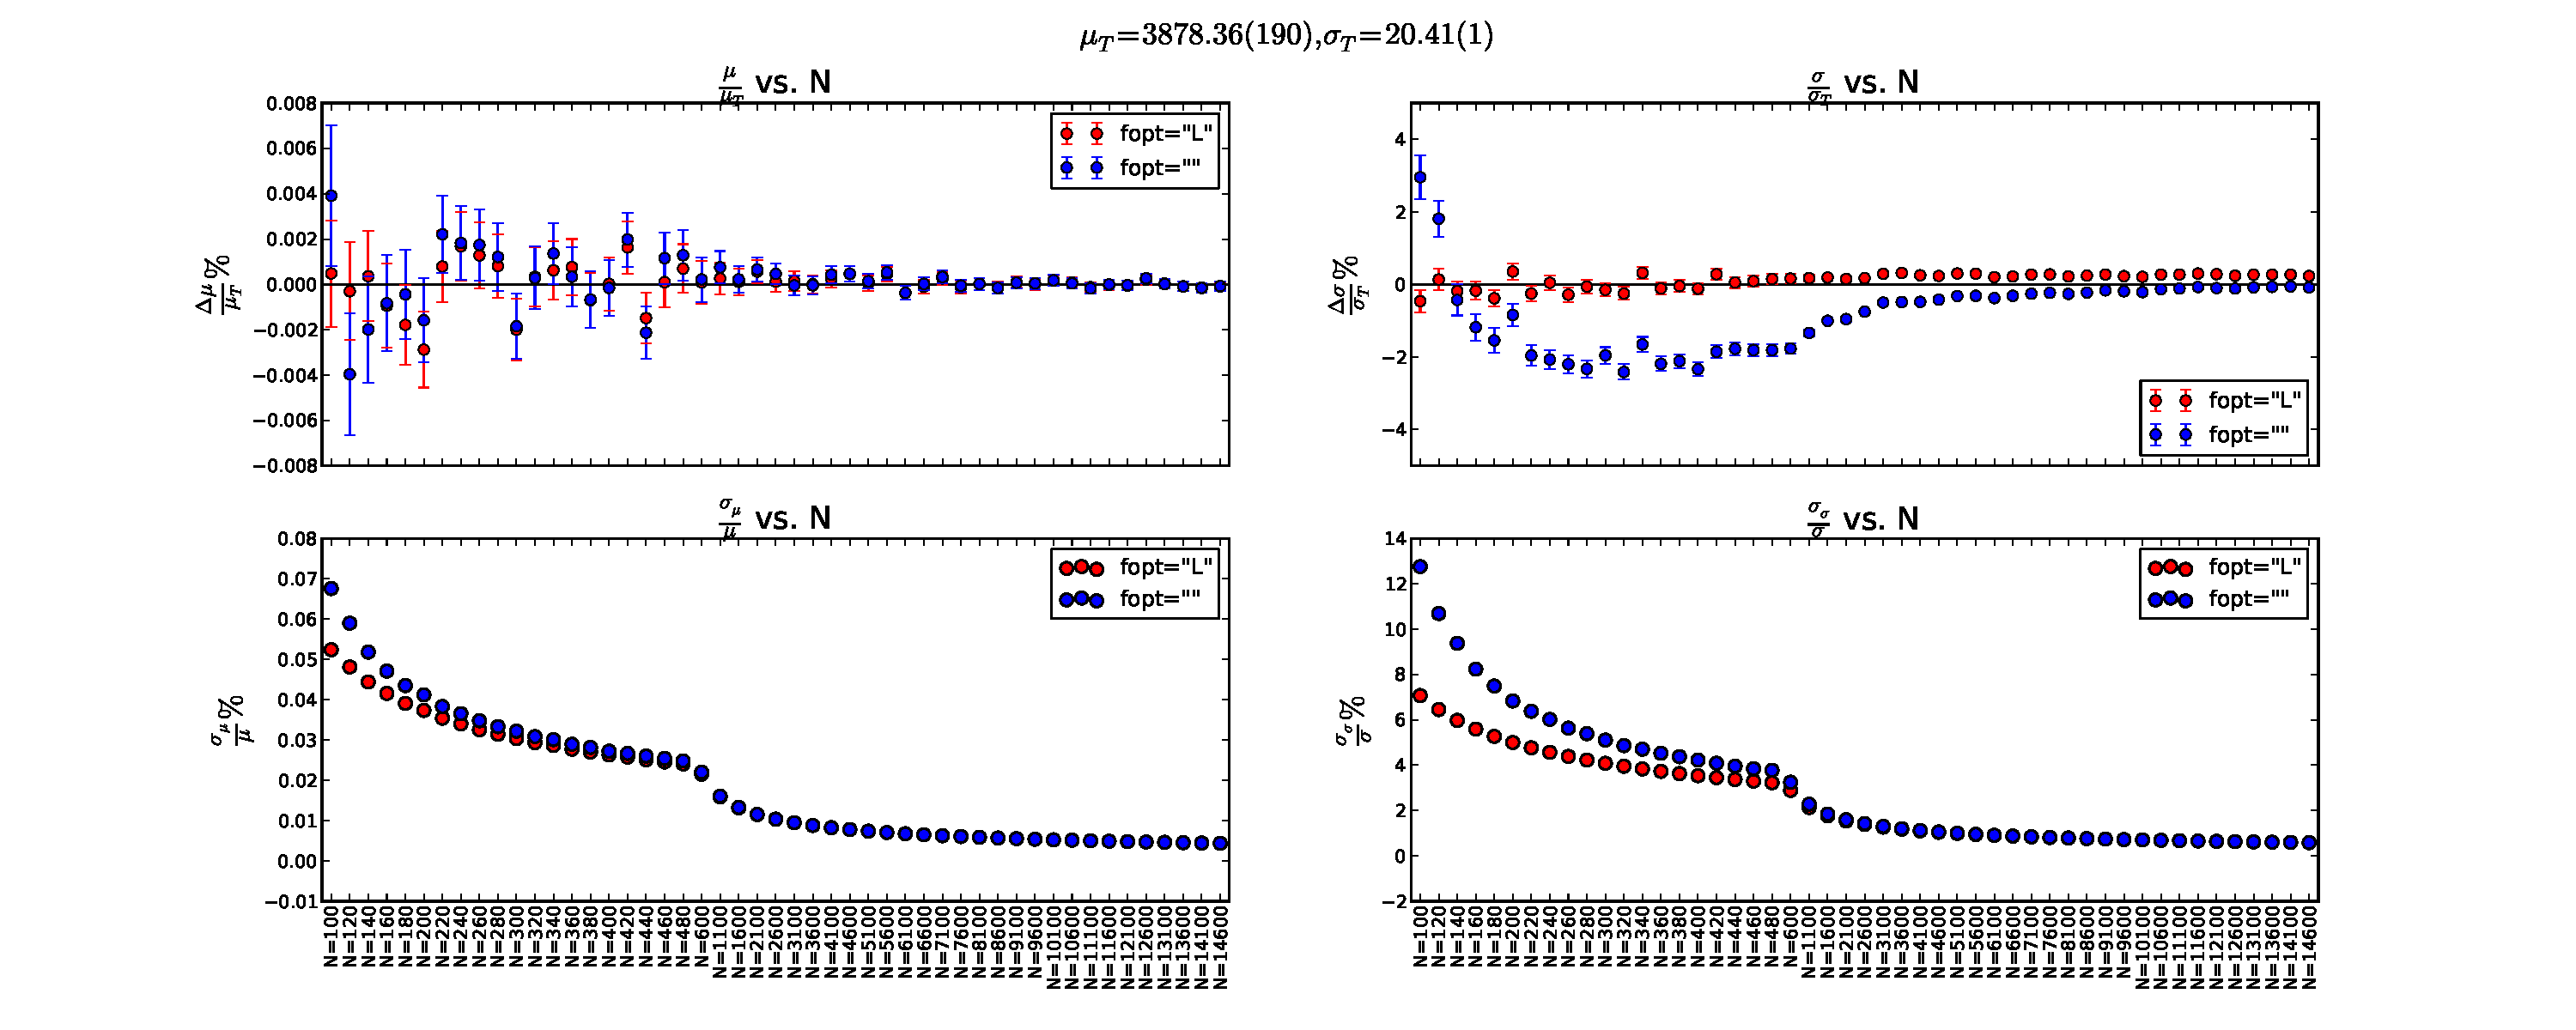
\includegraphics[height=2.5in,width=5.5in]{fit-comp_MU-190_SG-1_fit-opt-L_binw-025.pdf}
	%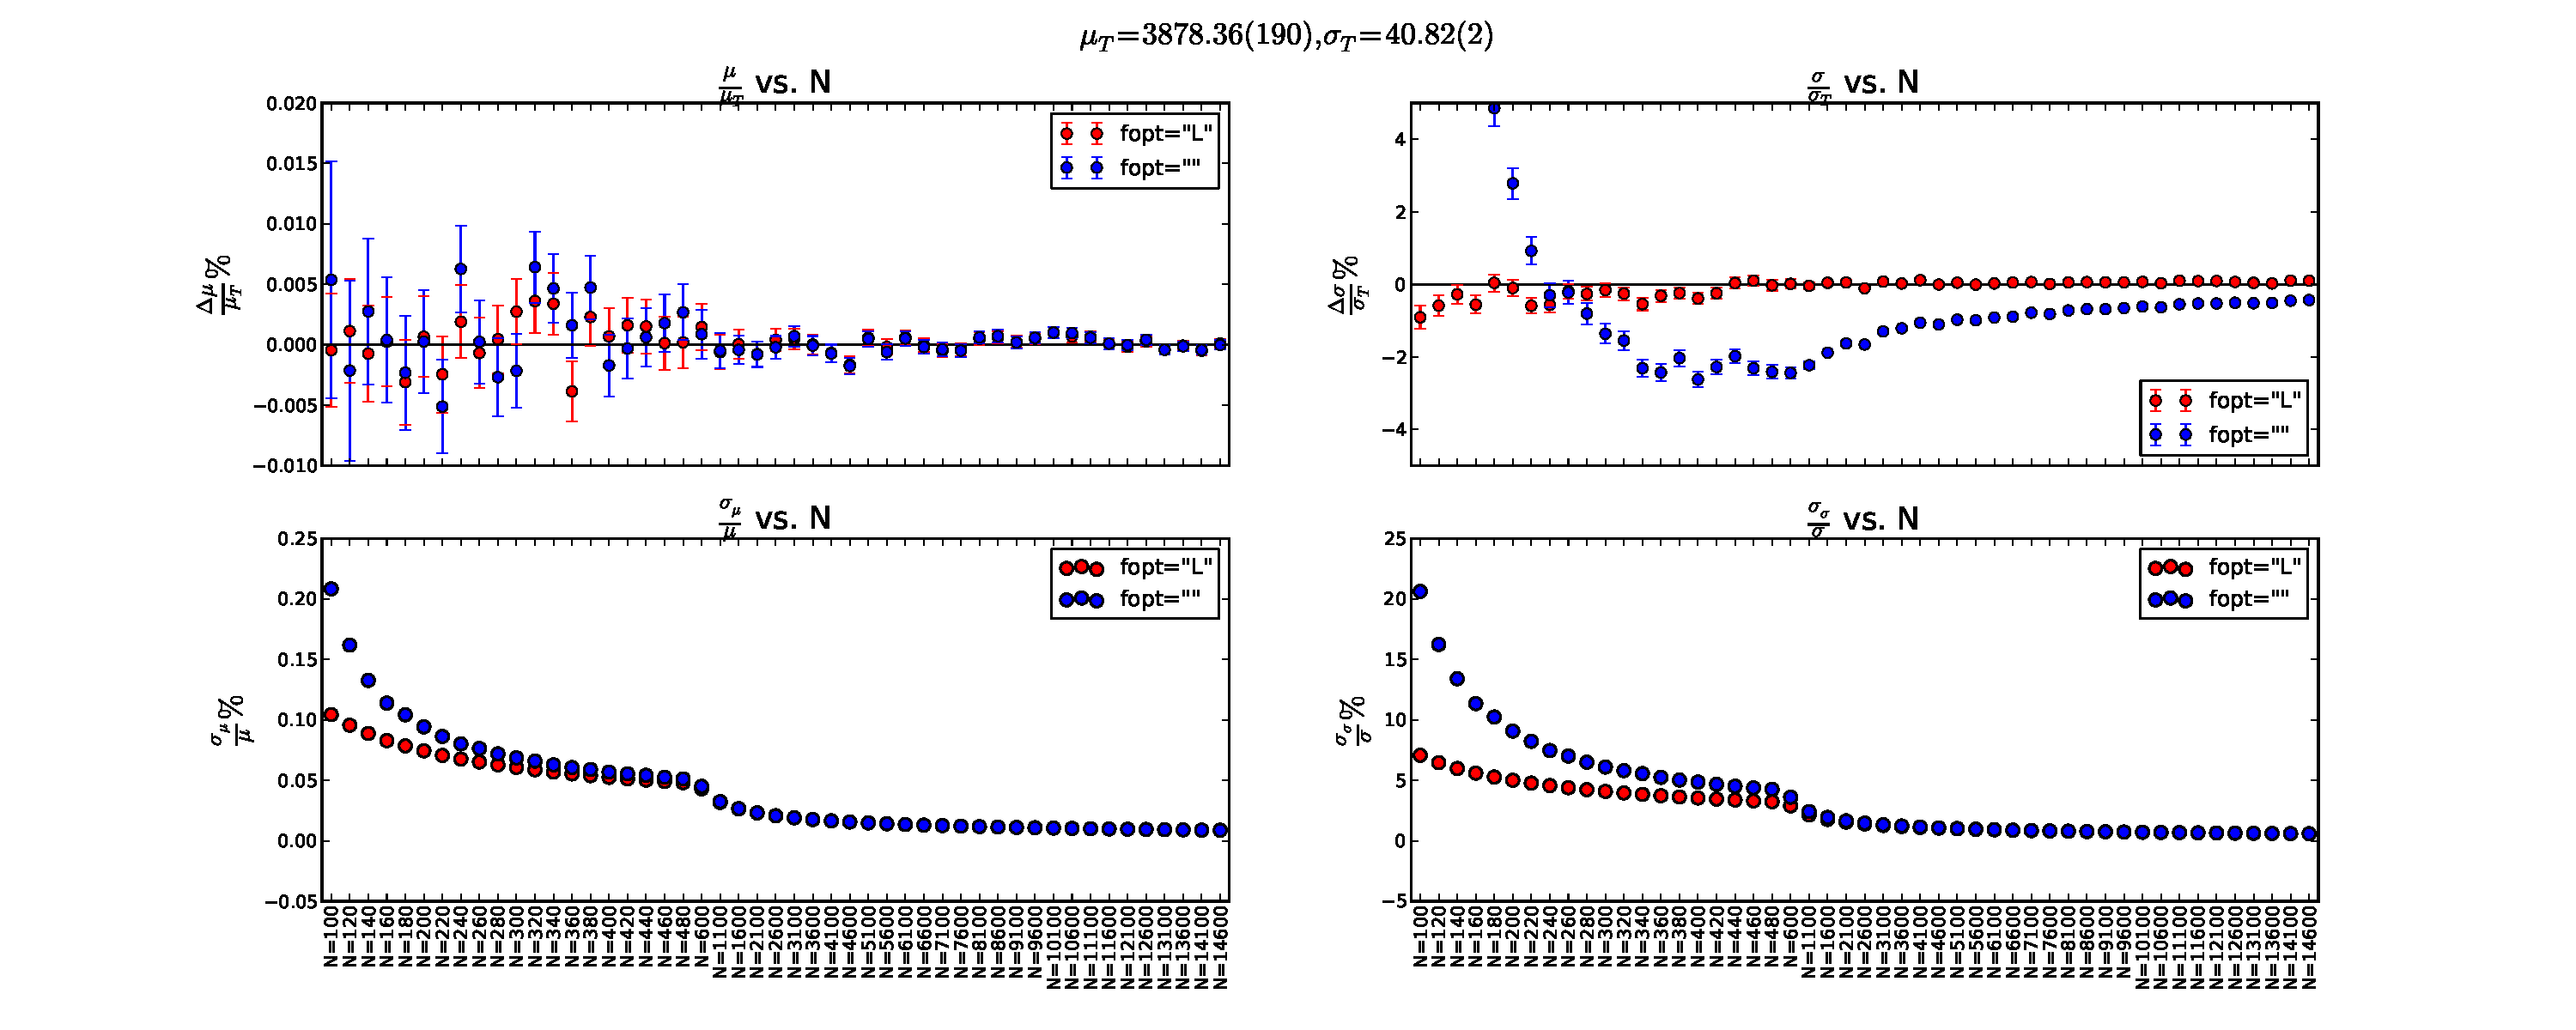
\includegraphics[height=2.5in,width=5.5in]{fit-comp_MU-190_SG-2_fit-opt-L_binw-025.pdf}
	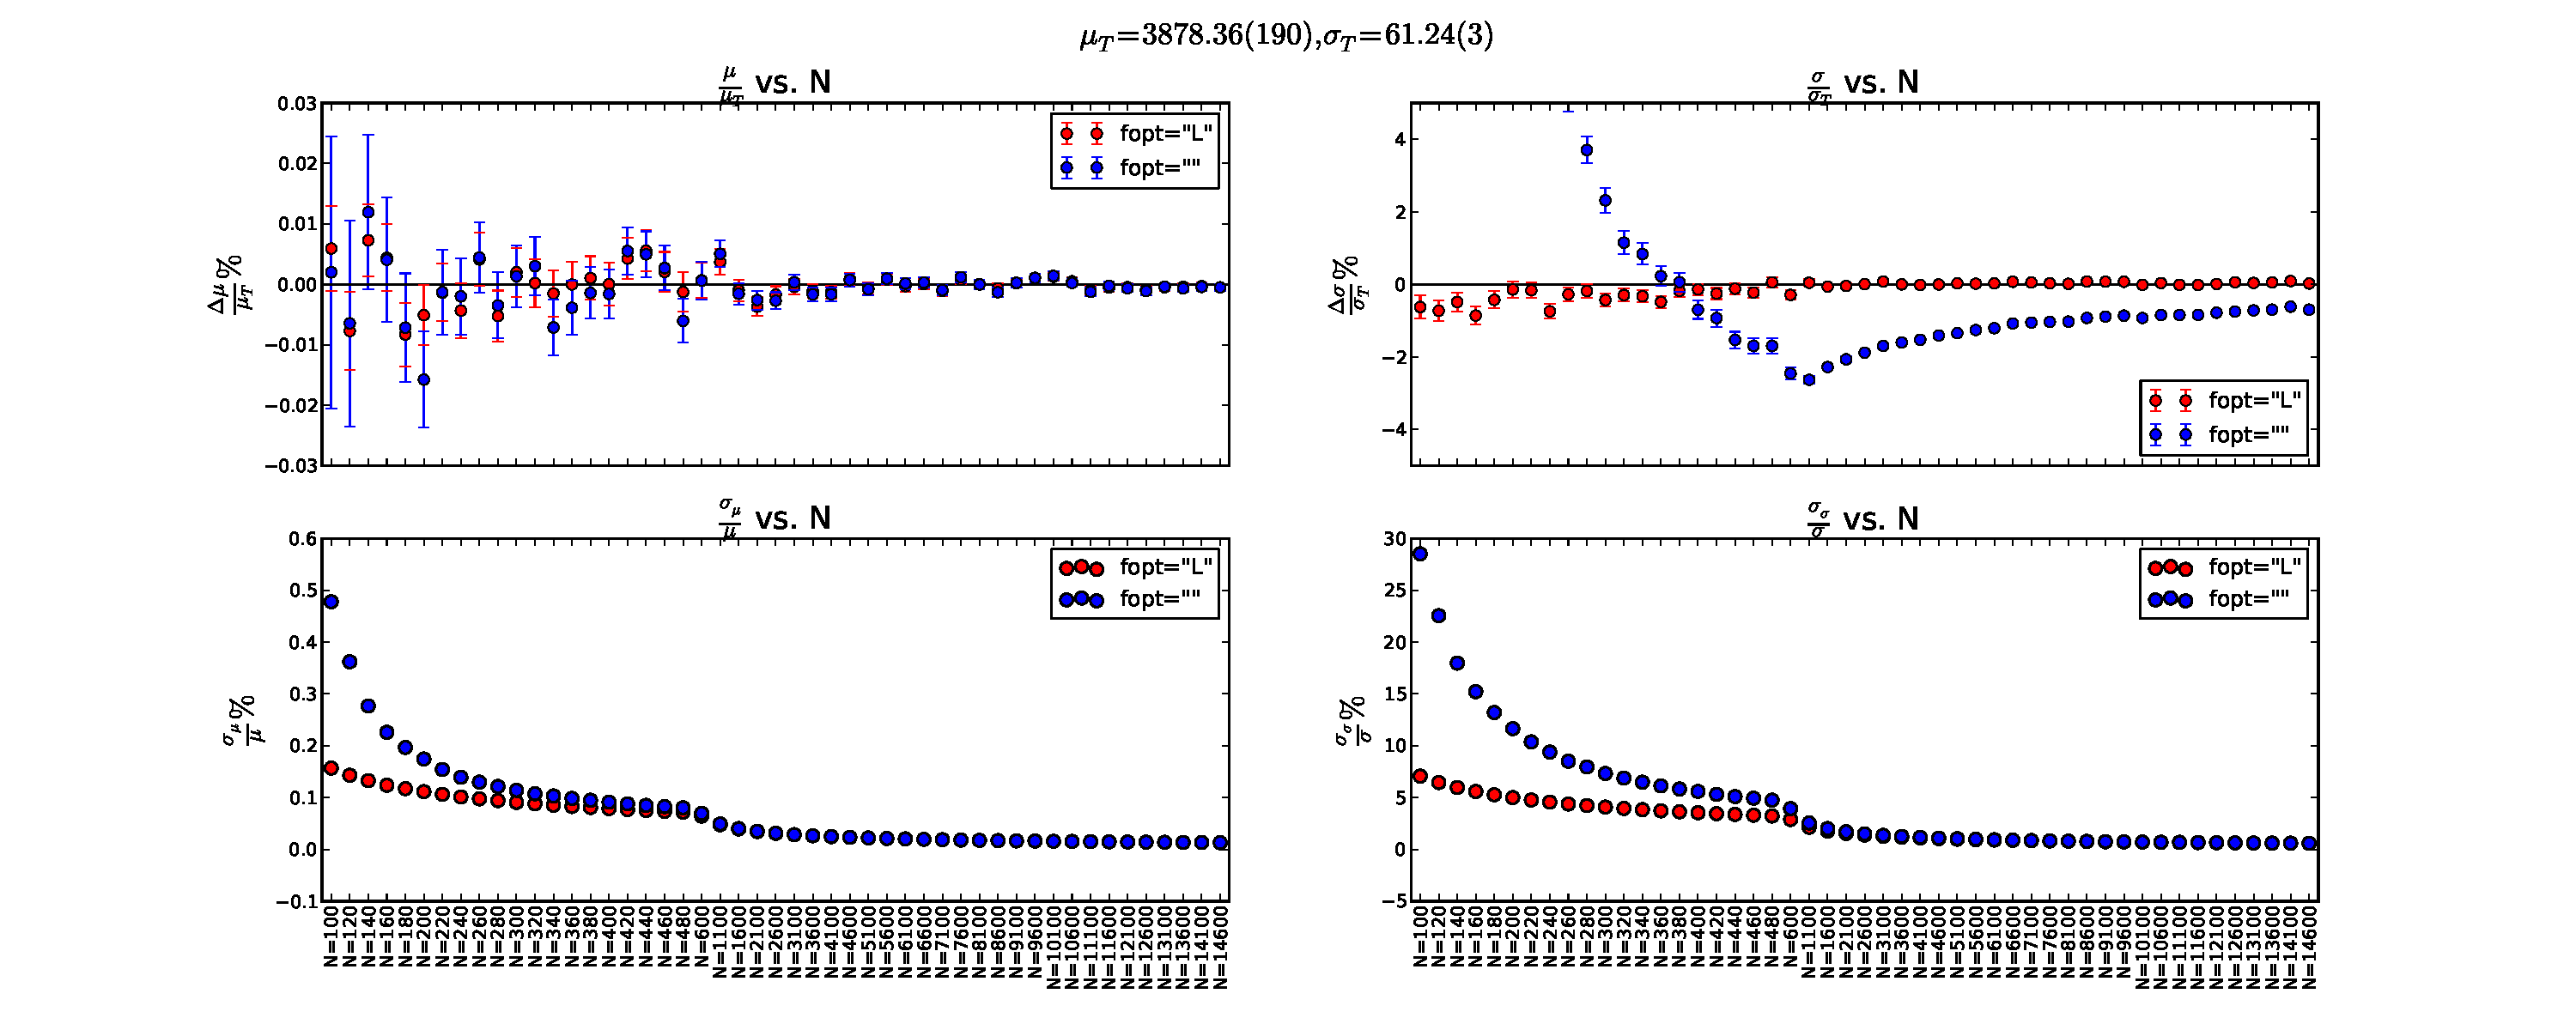
\includegraphics[height=2.5in,width=5.5in]{fit-comp_MU-190_SG-3_fit-opt-L_binw-025.pdf}
	%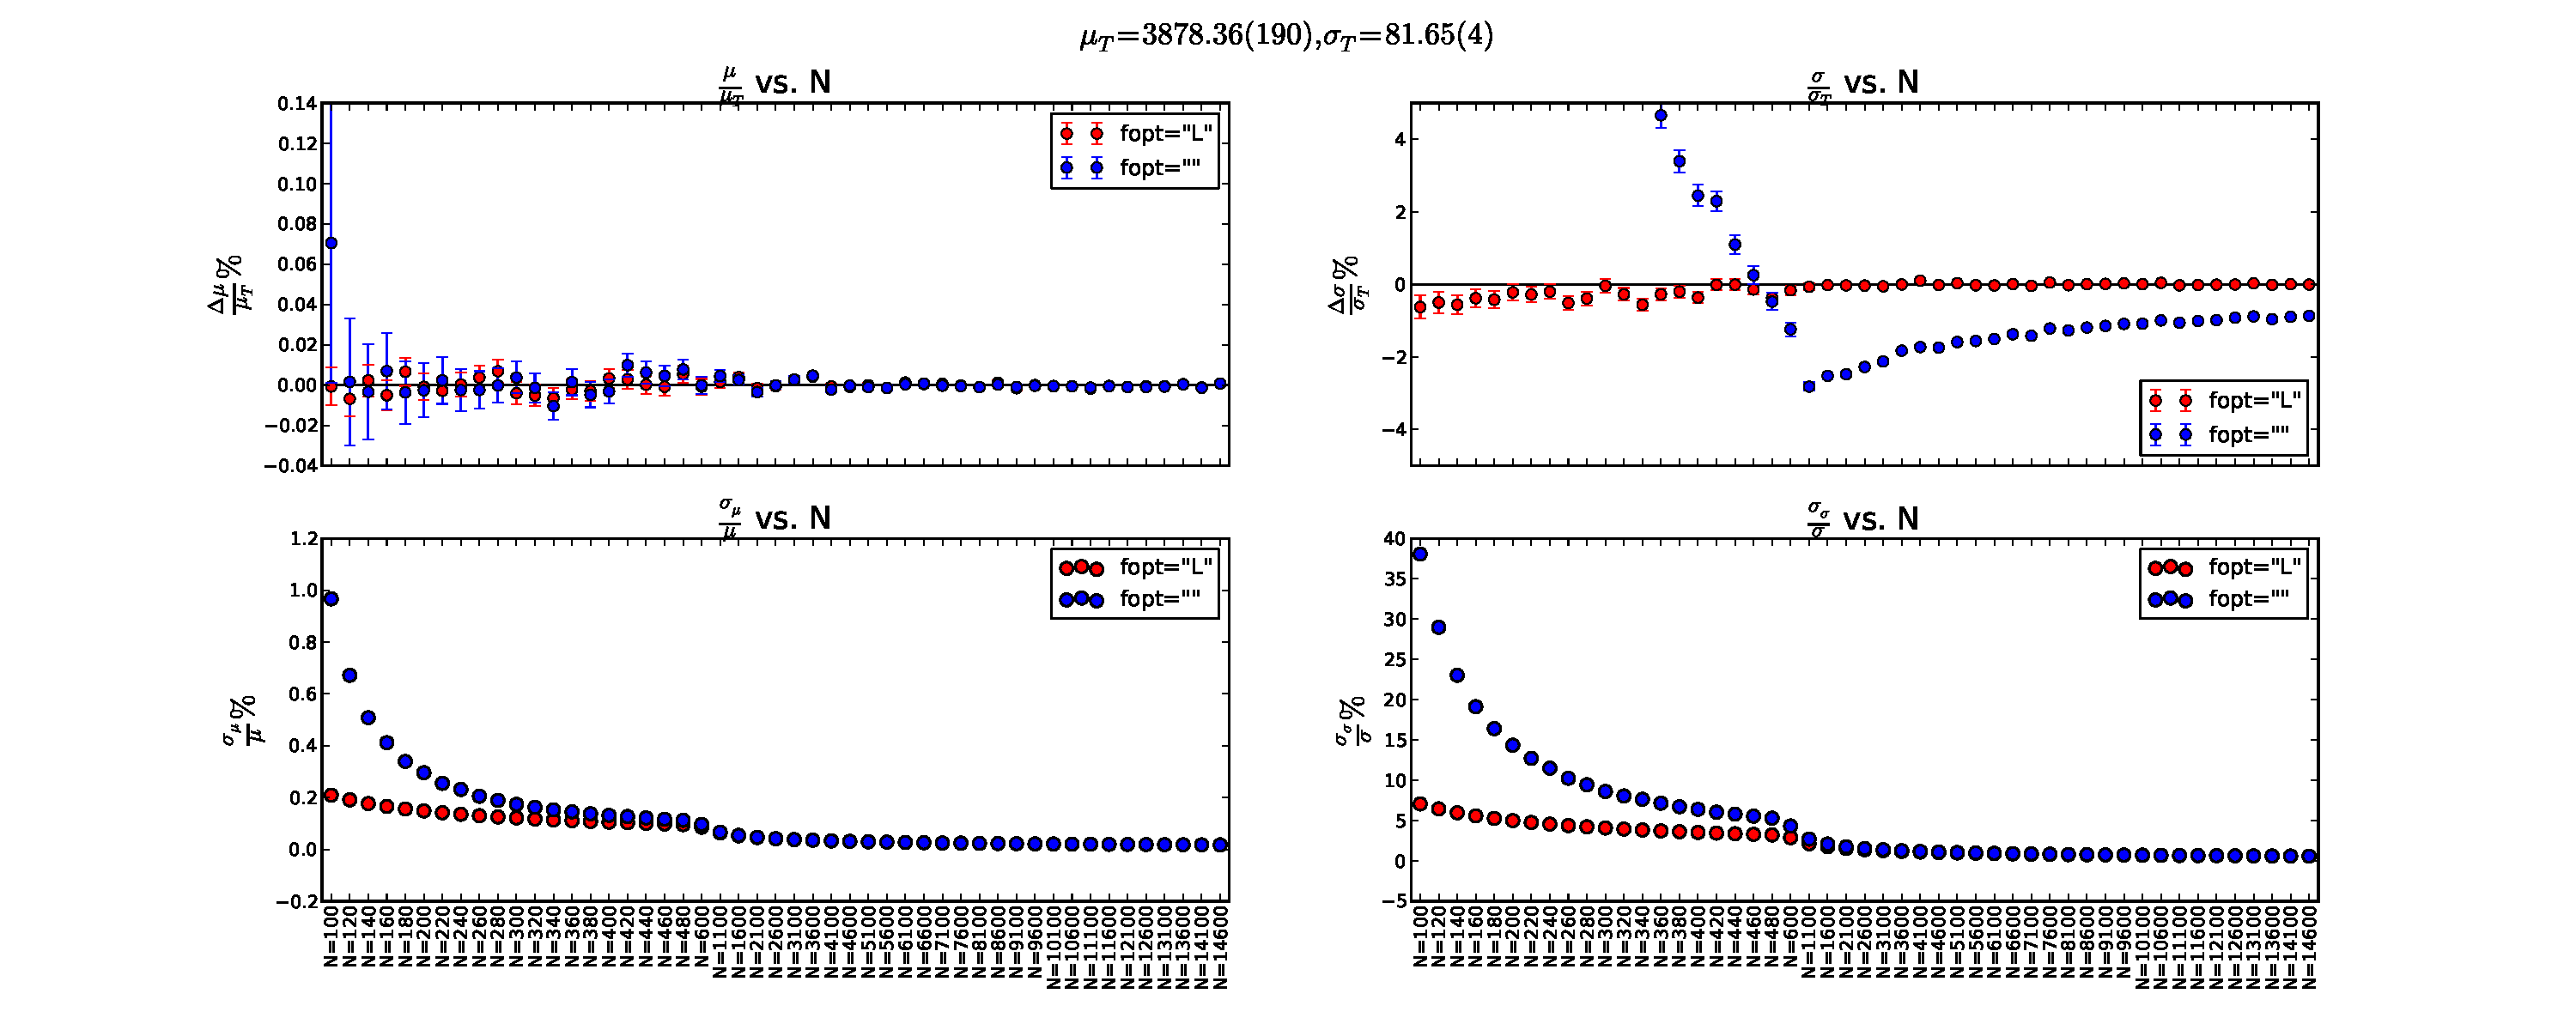
\includegraphics[height=2.5in,width=5.5in]{fit-comp_MU-190_SG-4_fit-opt-L_binw-025.pdf}
	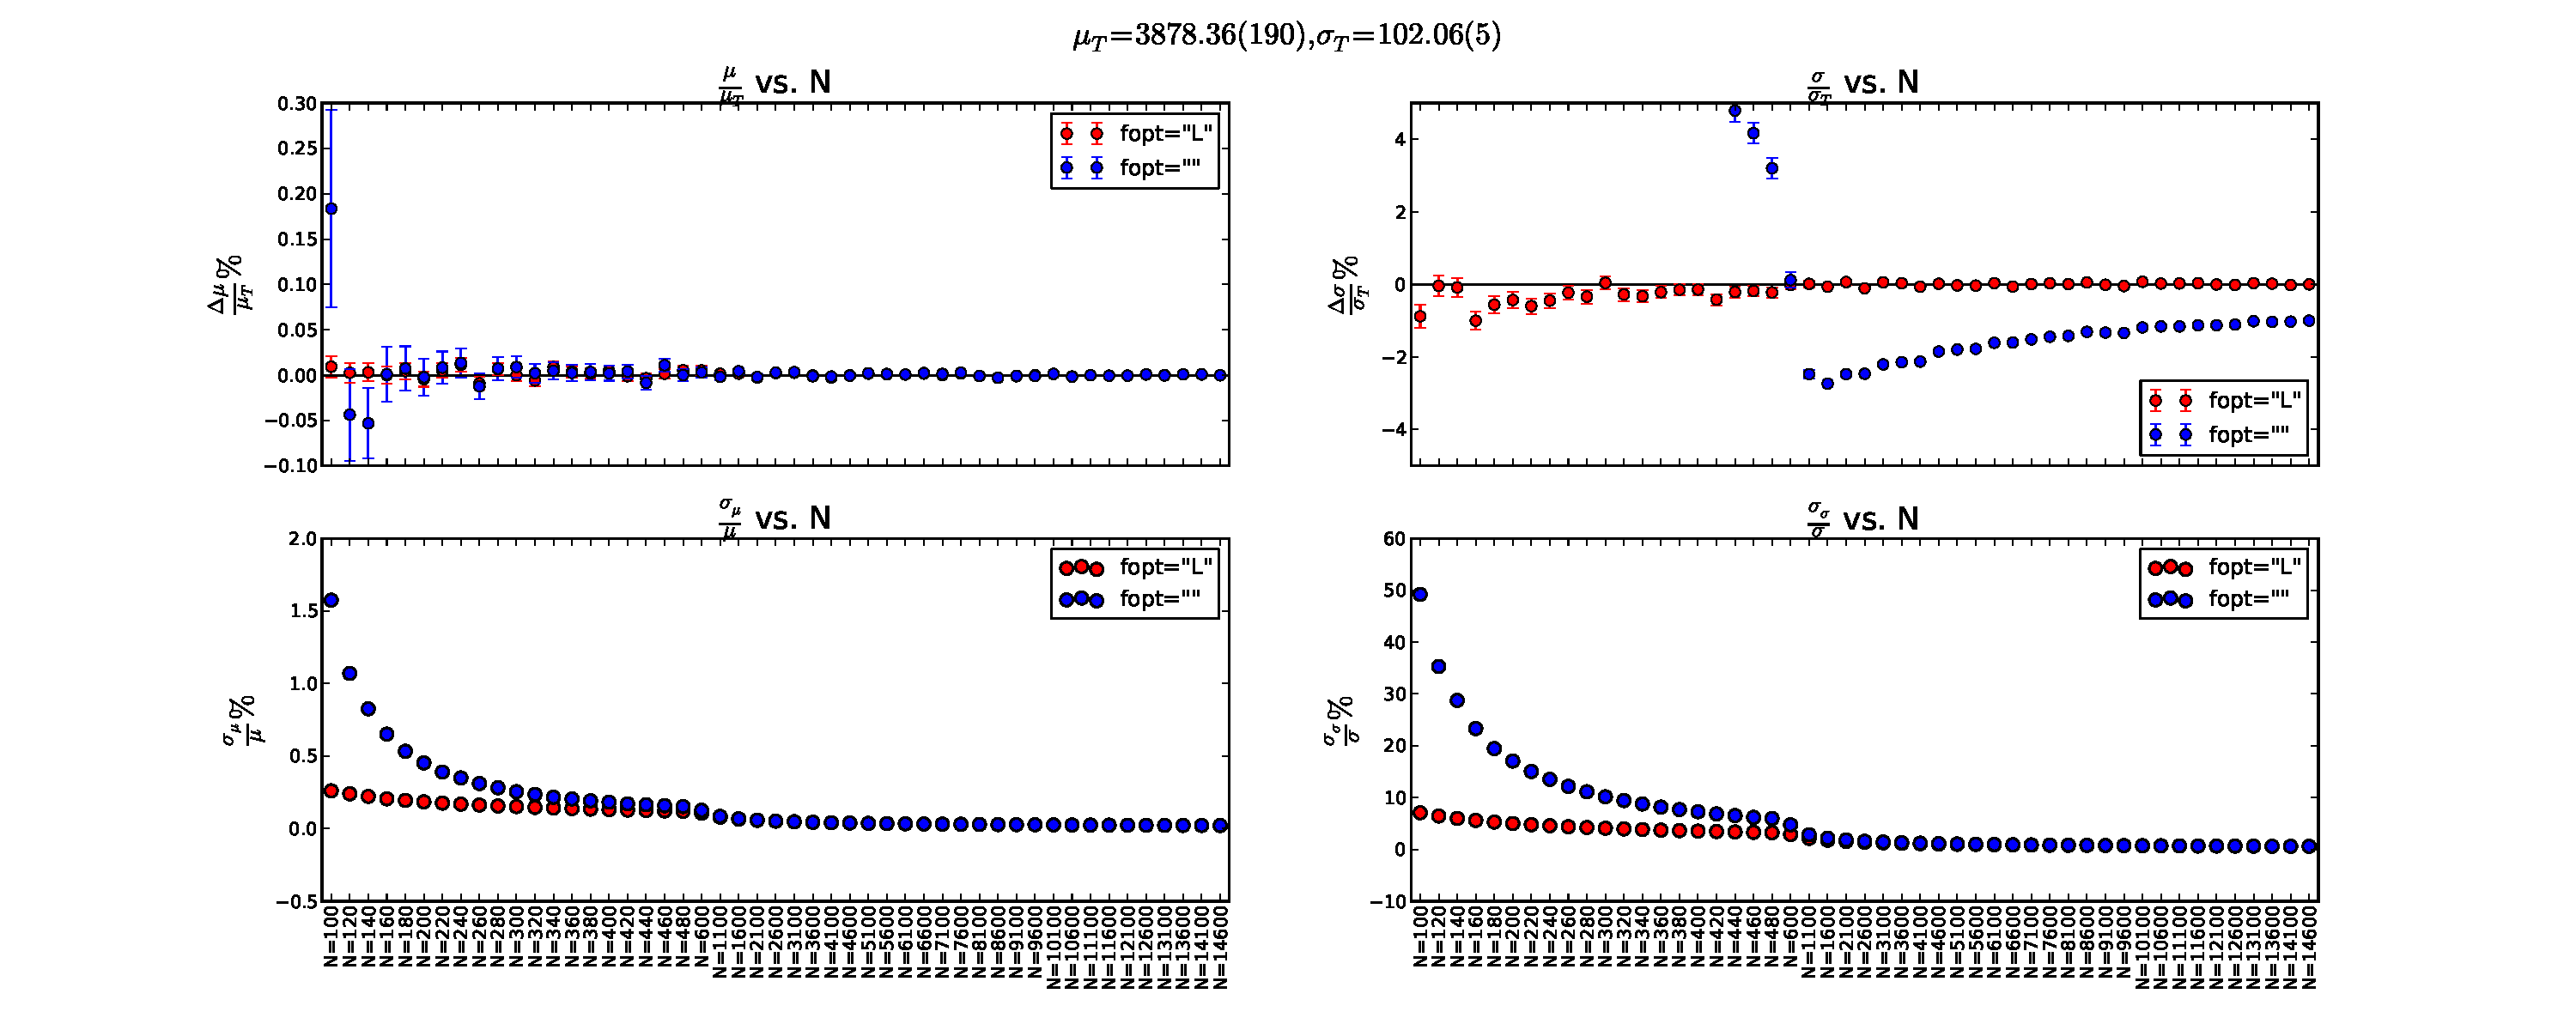
\includegraphics[height=2.5in,width=5.5in]{fit-comp_MU-190_SG-5_fit-opt-L_binw-025.pdf}
	\caption{Extracted parameters (MLE and CSQ) as a function of N and $\sigma_{T}$}
	\label{fig2}
\end{figure*}

\clearpage

From Fig. 2, it appears that regular Chi-square stastic(CSQ) is not suited for the level of statistics we have and therefore, the Maximum Likelihood(MLE) fit will best serve our purpose. However, the MLE option is also not suited for our purpose because the fit is more sensitive to points that lie beyond the expected limits of the T-distribution (``bad track?'') and therefore returns a higher value for the standard devitation. The other remaining option is to use CSQ-WW (set weights in all bins to 1 and ignore error bars), which behaves like MLE, but it is slightly more biased for low N and the statistical error bars are underestimated. Fig. 3 shows the extracted parameters from the CSQ-WW option (compared with CSQ)

\begin{figure*}[ht]
	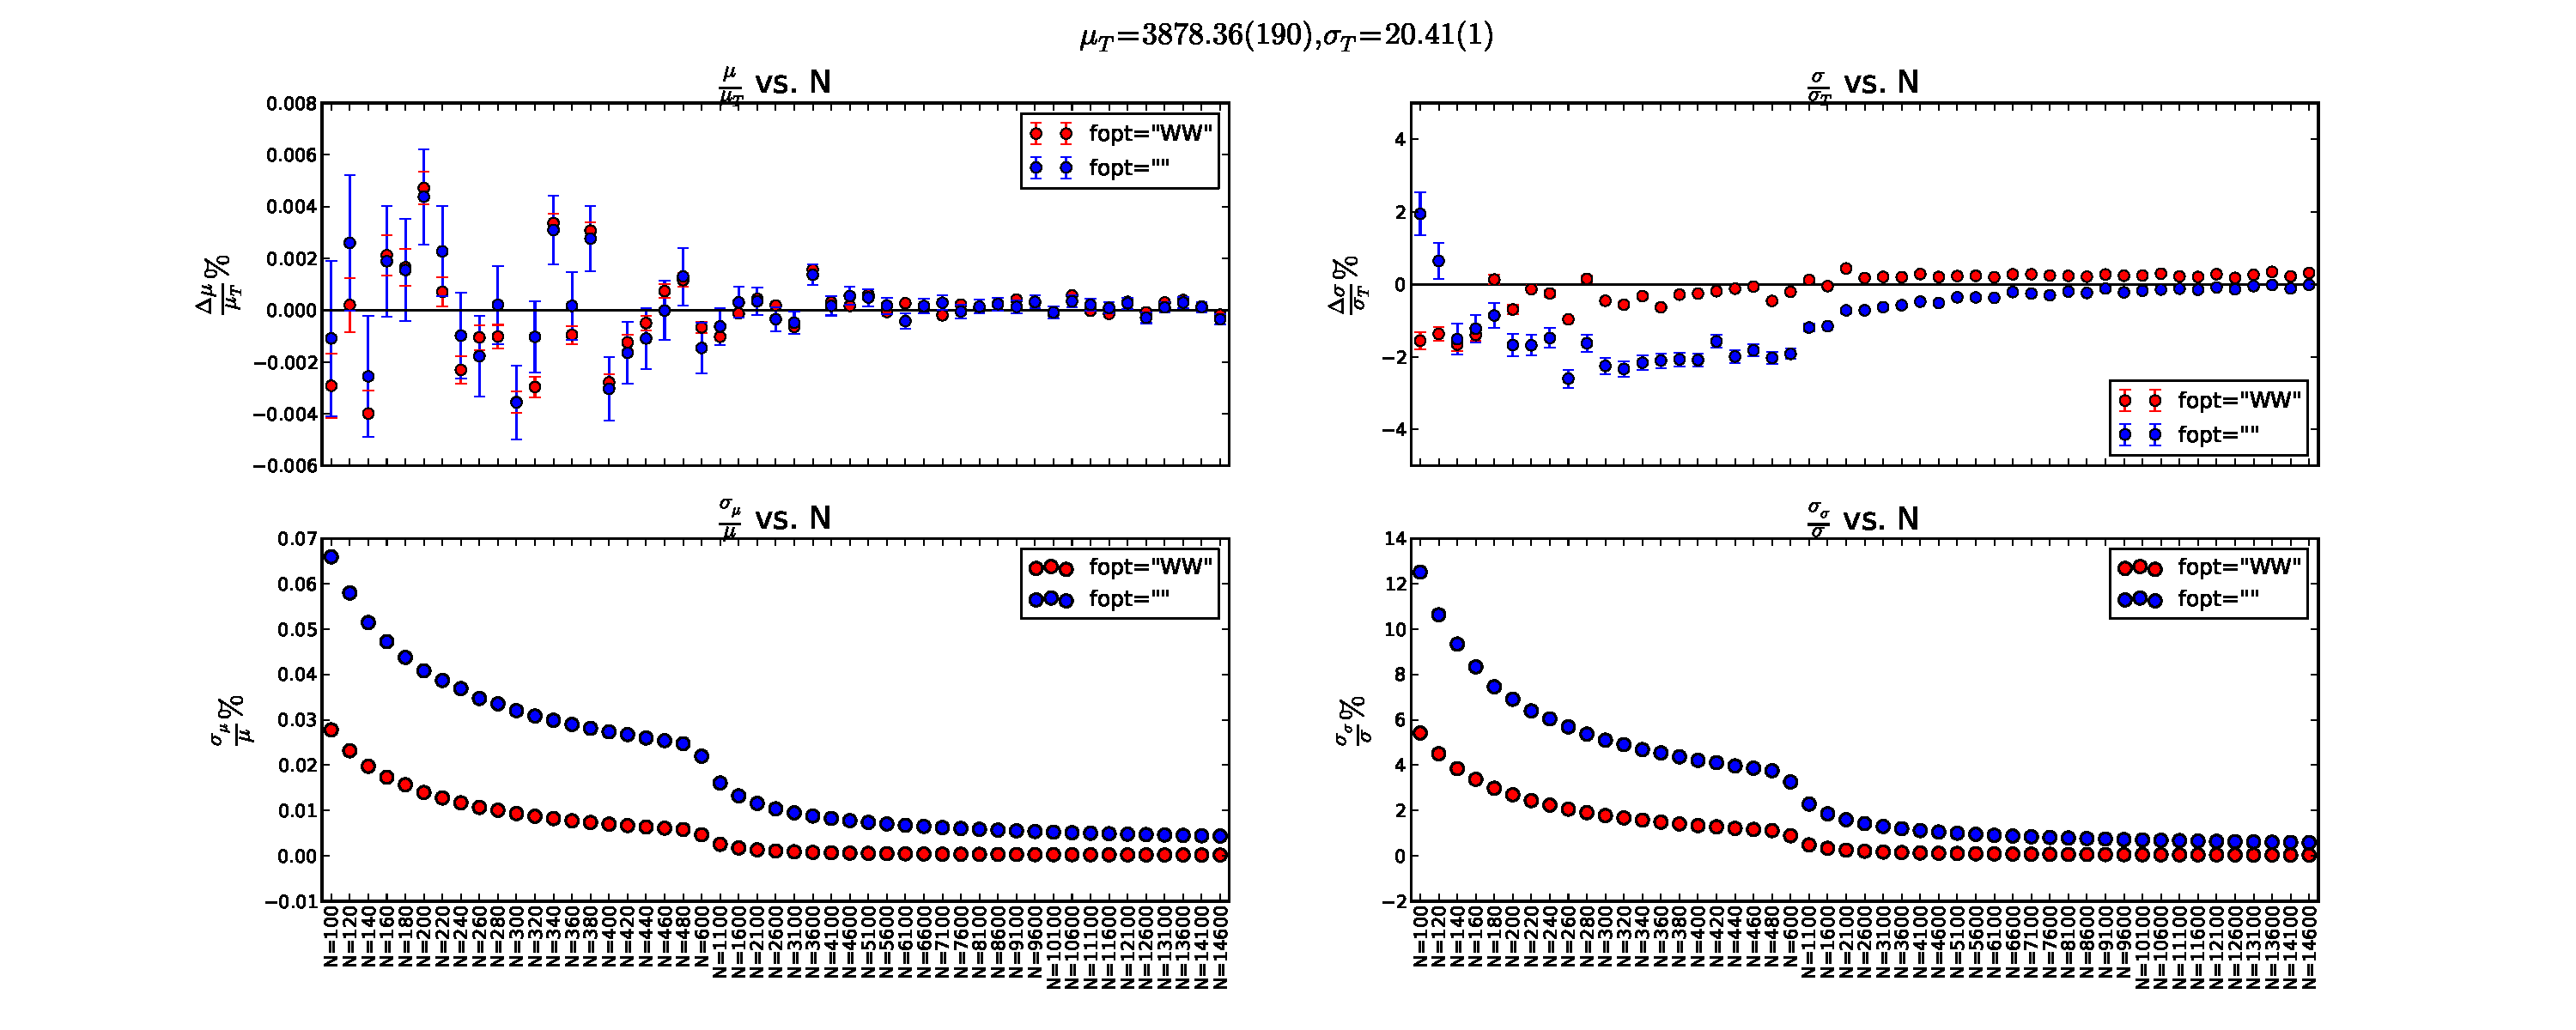
\includegraphics[height=2.5in,width=5.5in]{fit-comp_MU-190_SG-1_fit-opt-WW_binw-025.pdf}
	%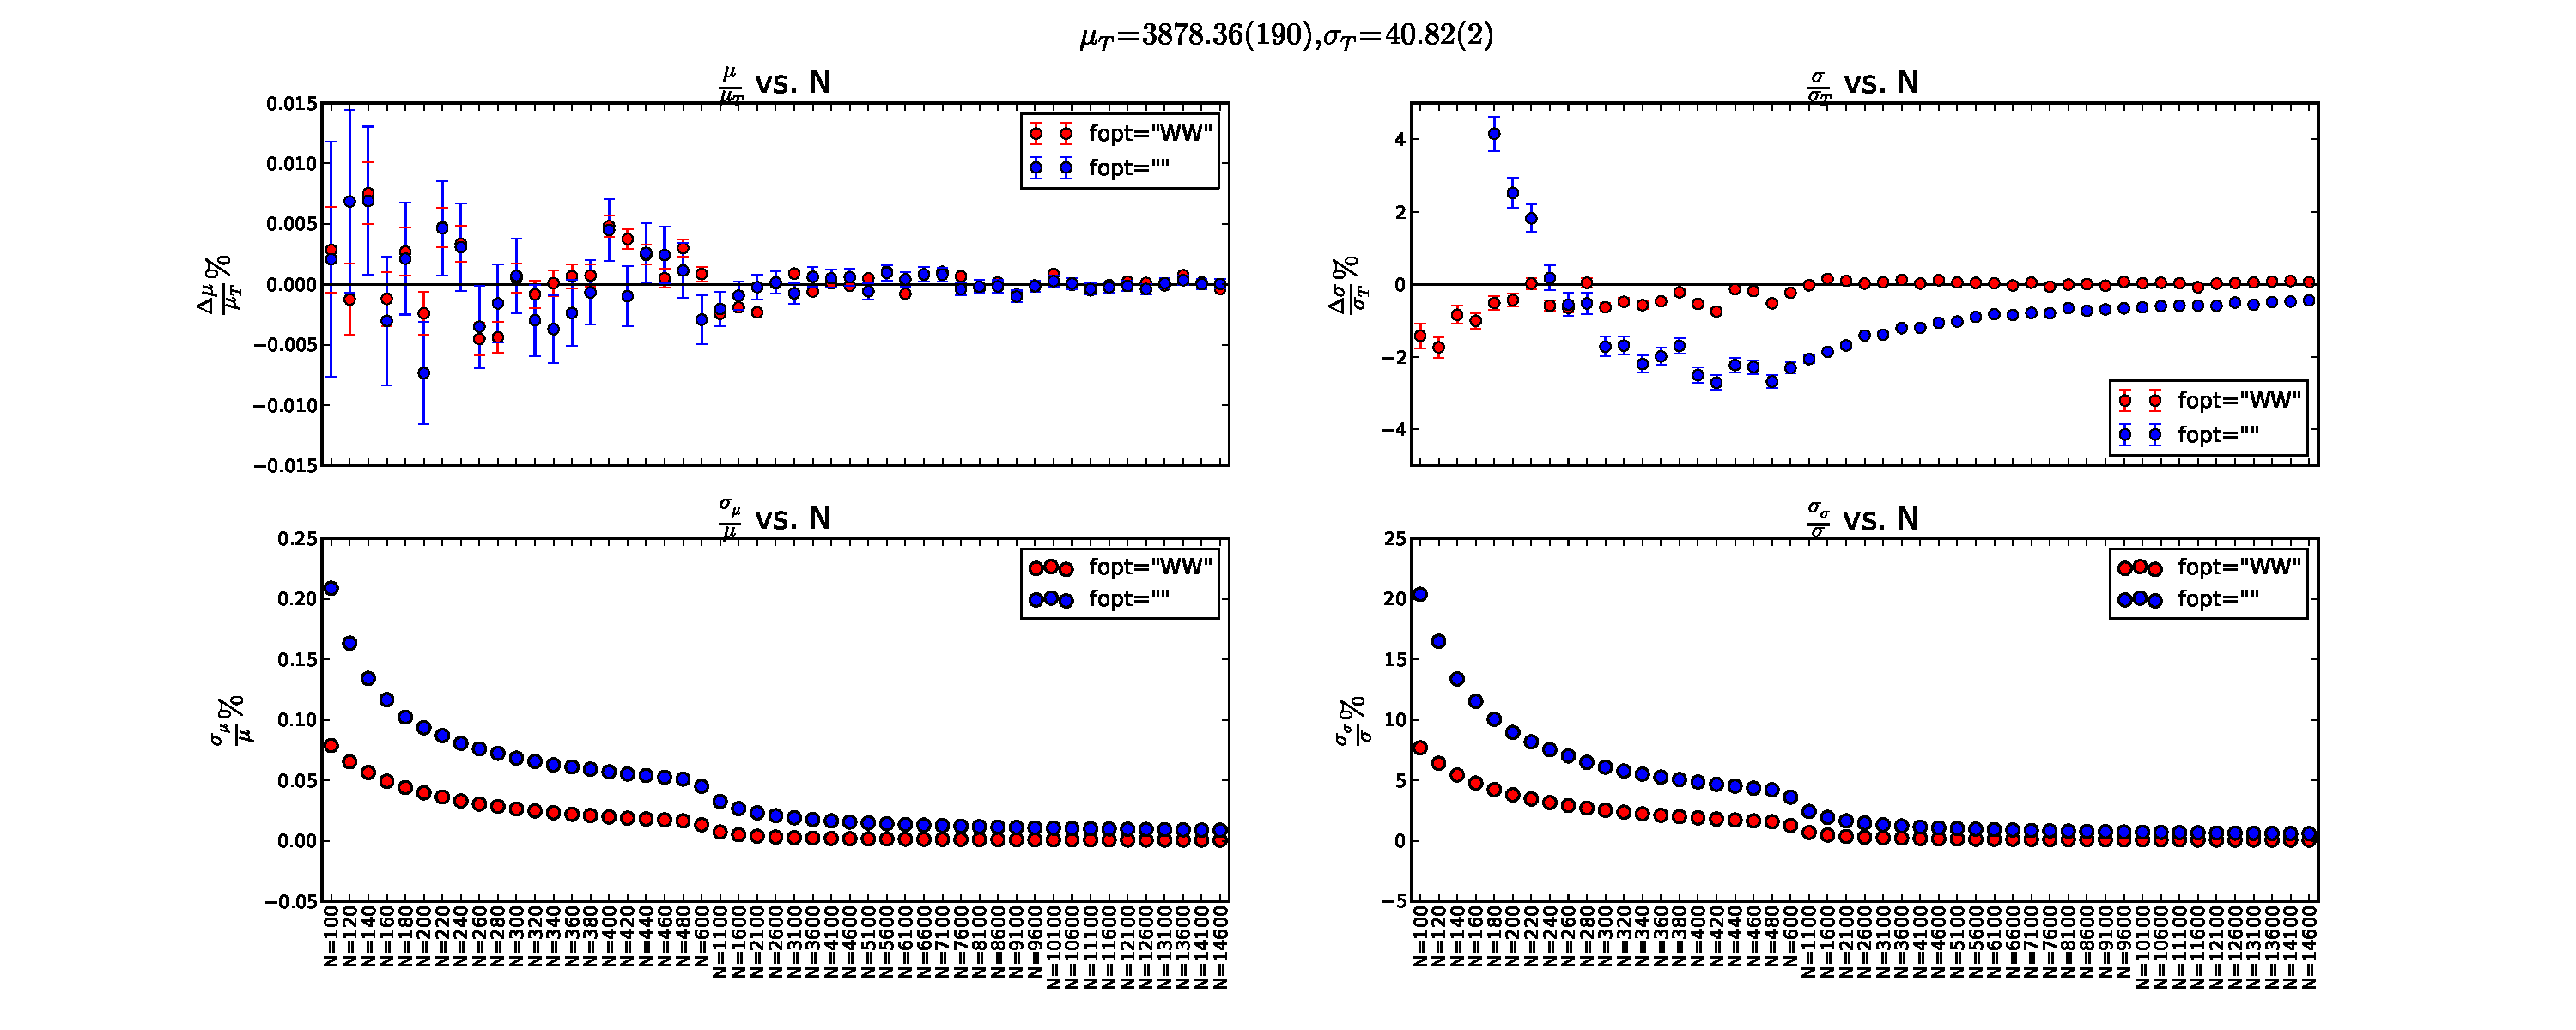
\includegraphics[height=2.5in,width=5.5in]{fit-comp_MU-190_SG-2_fit-opt-WW_binw-025.pdf}
	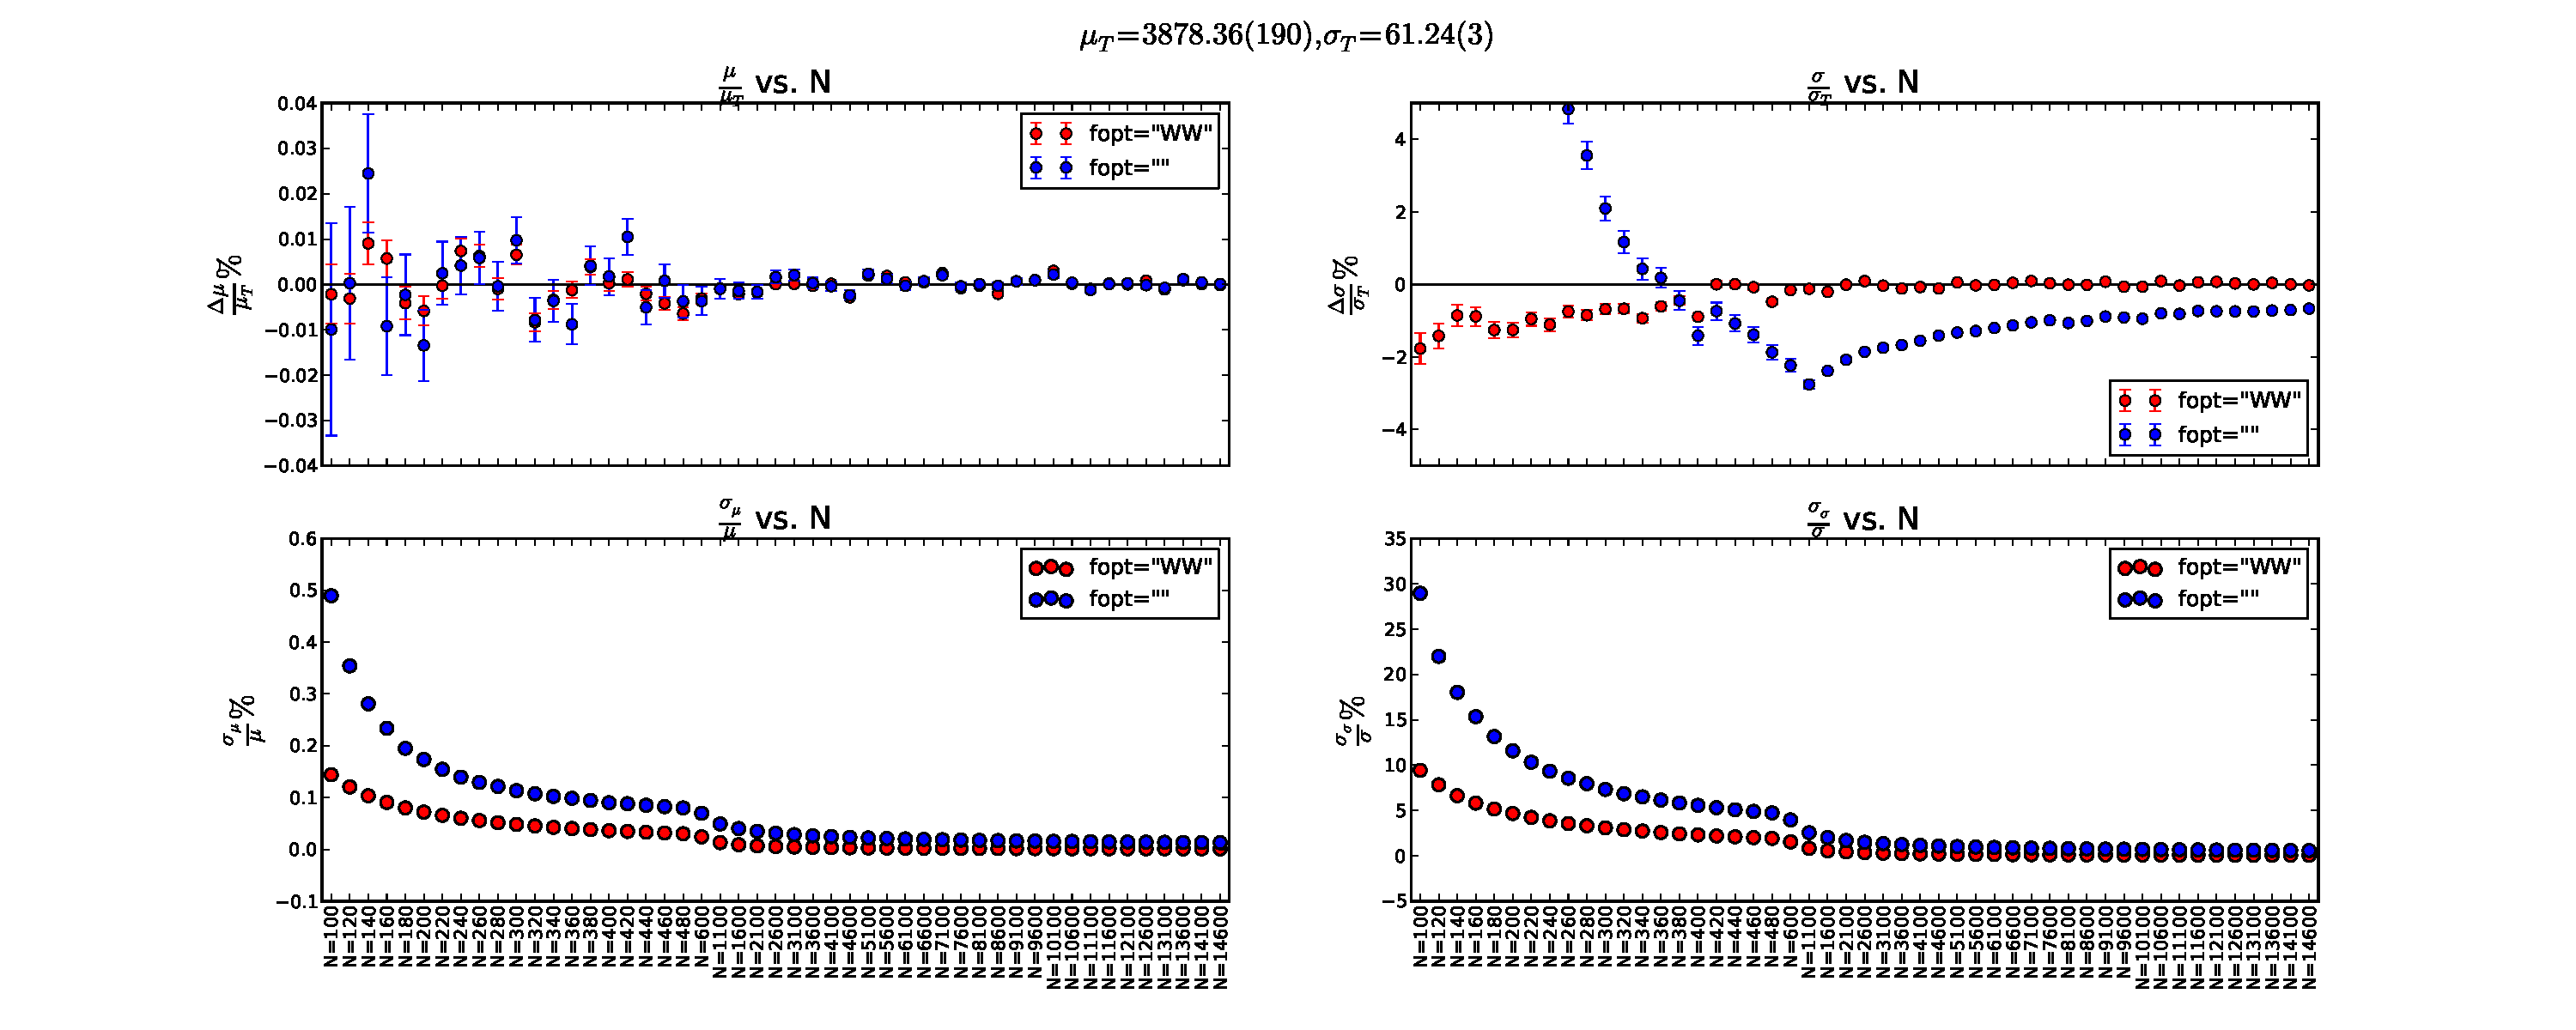
\includegraphics[height=2.5in,width=5.5in]{fit-comp_MU-190_SG-3_fit-opt-WW_binw-025.pdf}
	%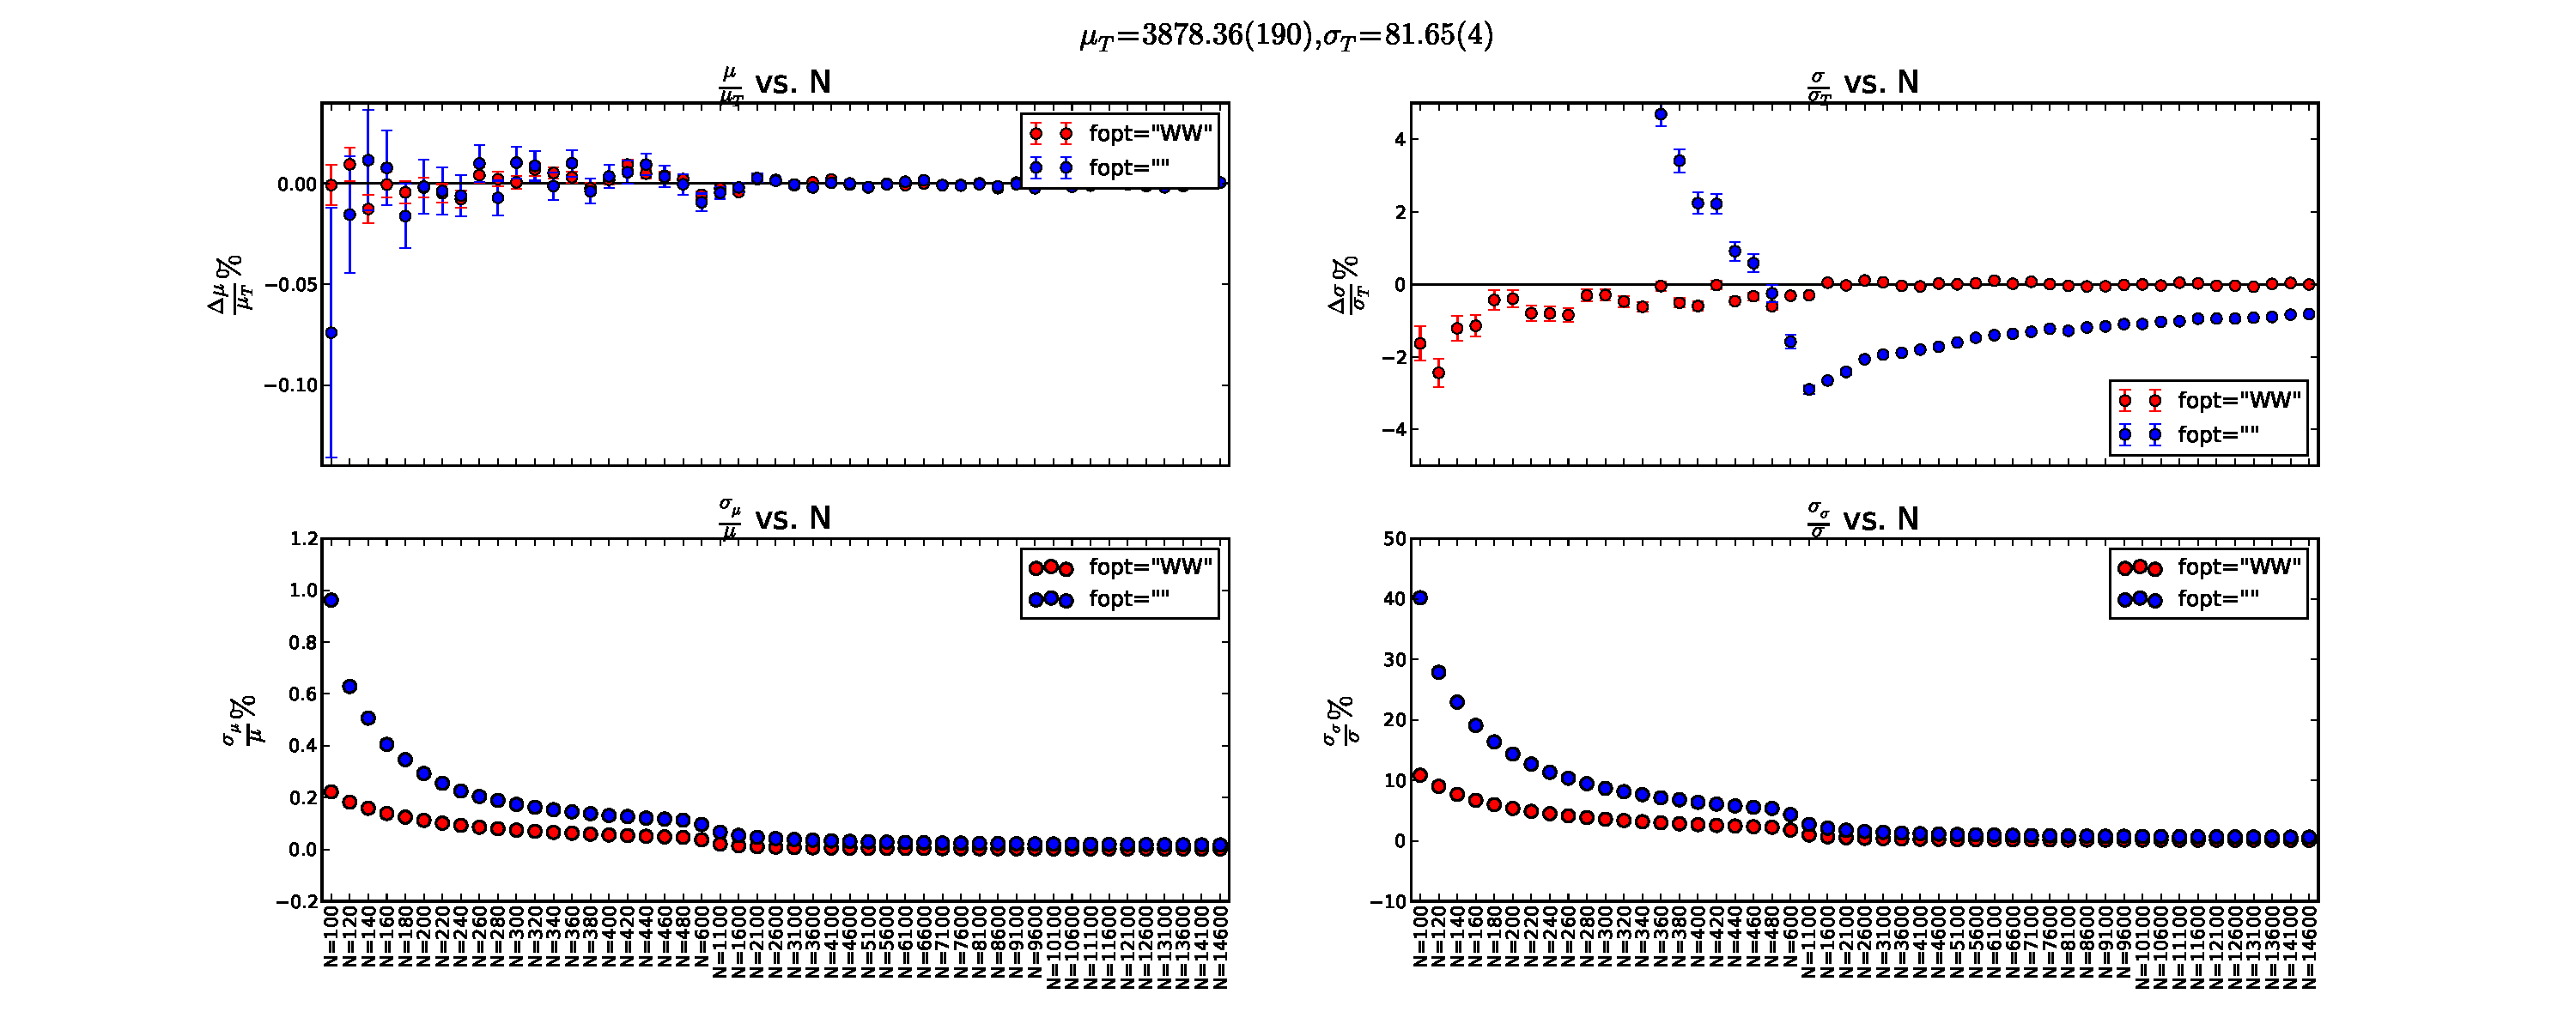
\includegraphics[height=2.5in,width=5.5in]{fit-comp_MU-190_SG-4_fit-opt-WW_binw-025.pdf}
	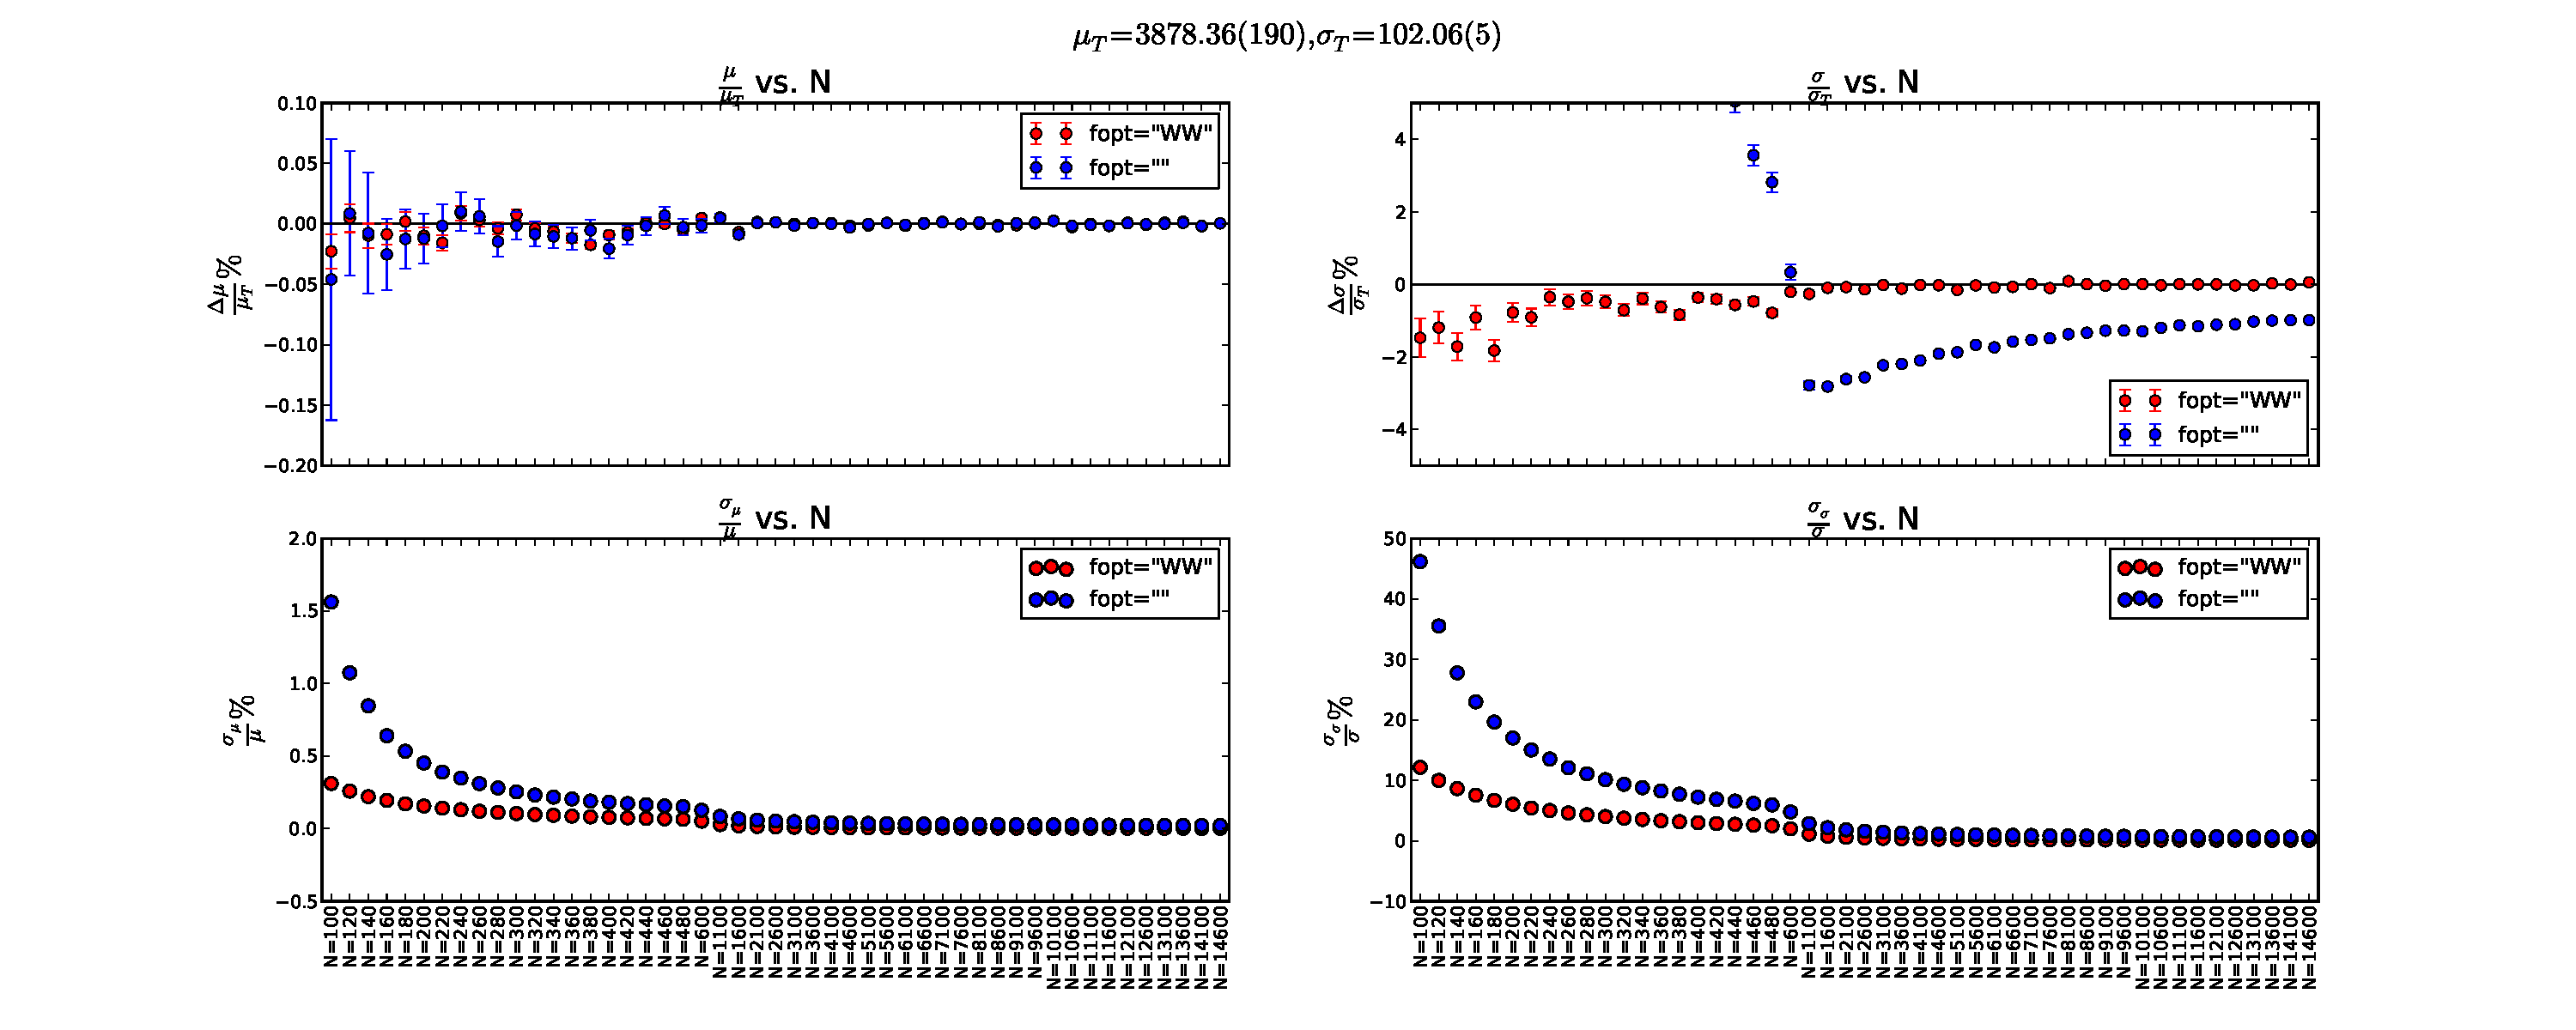
\includegraphics[height=2.5in,width=5.5in]{fit-comp_MU-190_SG-5_fit-opt-WW_binw-025.pdf}
	\caption{Extracted parameters (CSQWW and CSQ)as a function of N and $\sigma_{T}$}
	\label{fig3}
\end{figure*}

\clearpage

Following is the summary of the different ROOT Fit methods compared and their performance at low N (see Fig. 6 for a plot comparing the time resolution obtained from each):

\begin{itemize}
	\item CSQ: Highly based at low N
	\item MLE: Susceptible to ``bad tracks''
	\item CSQWW: Slightly more biased than MLE and reduced statistical errors. 
\end{itemize}

Therefore, given the statistics and the need to efficiently optimize the automation program, it is best to use the CSQ-WW Fit, even though the statistical errors are underestimated. The following figure illustrates this underestimation of errors.

\begin{figure*}[ht]
	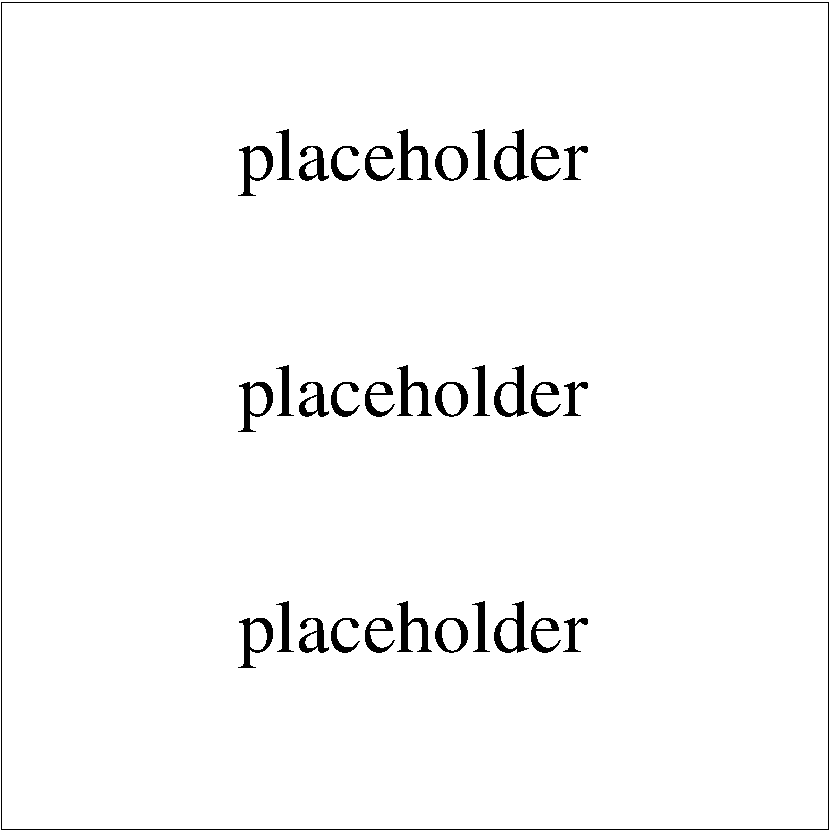
\includegraphics[height=2.5in,width=5.5in]{placeholder.pdf}
	\caption{Demo underestimation of errors by CSQWW by comparing with MLE by way of resolution vs. point plot (I had previously compared with CSQ, but with binw=0.25, CSQ is no longer valid to compare with if sets with binw=0.25 is to be used) }
	\label{fig4}
\end{figure*}

However, this underestimation of errors per point is not a concern because ultimately we work with the average resolution of the bar and in the process, the averaged statistical error estimate is significantly reduced and additionally, compared to the ``systematic error'' of 1 ps, is negligible(estimated from 40-dr-2dc for 210cm, 1st-article counters; I think it will vary between sets and get higher for longer bars). (``systematic error'' $\defeq$ due to variation in TW parameters used to construct T and therefore of the time-resolution;anything else?)

Fig. 5 shows the statistical errors for $\langle res\_2\_3\_4 \rangle$ (from Normal Order) for various bar lengths

\begin{figure*}[ht]
	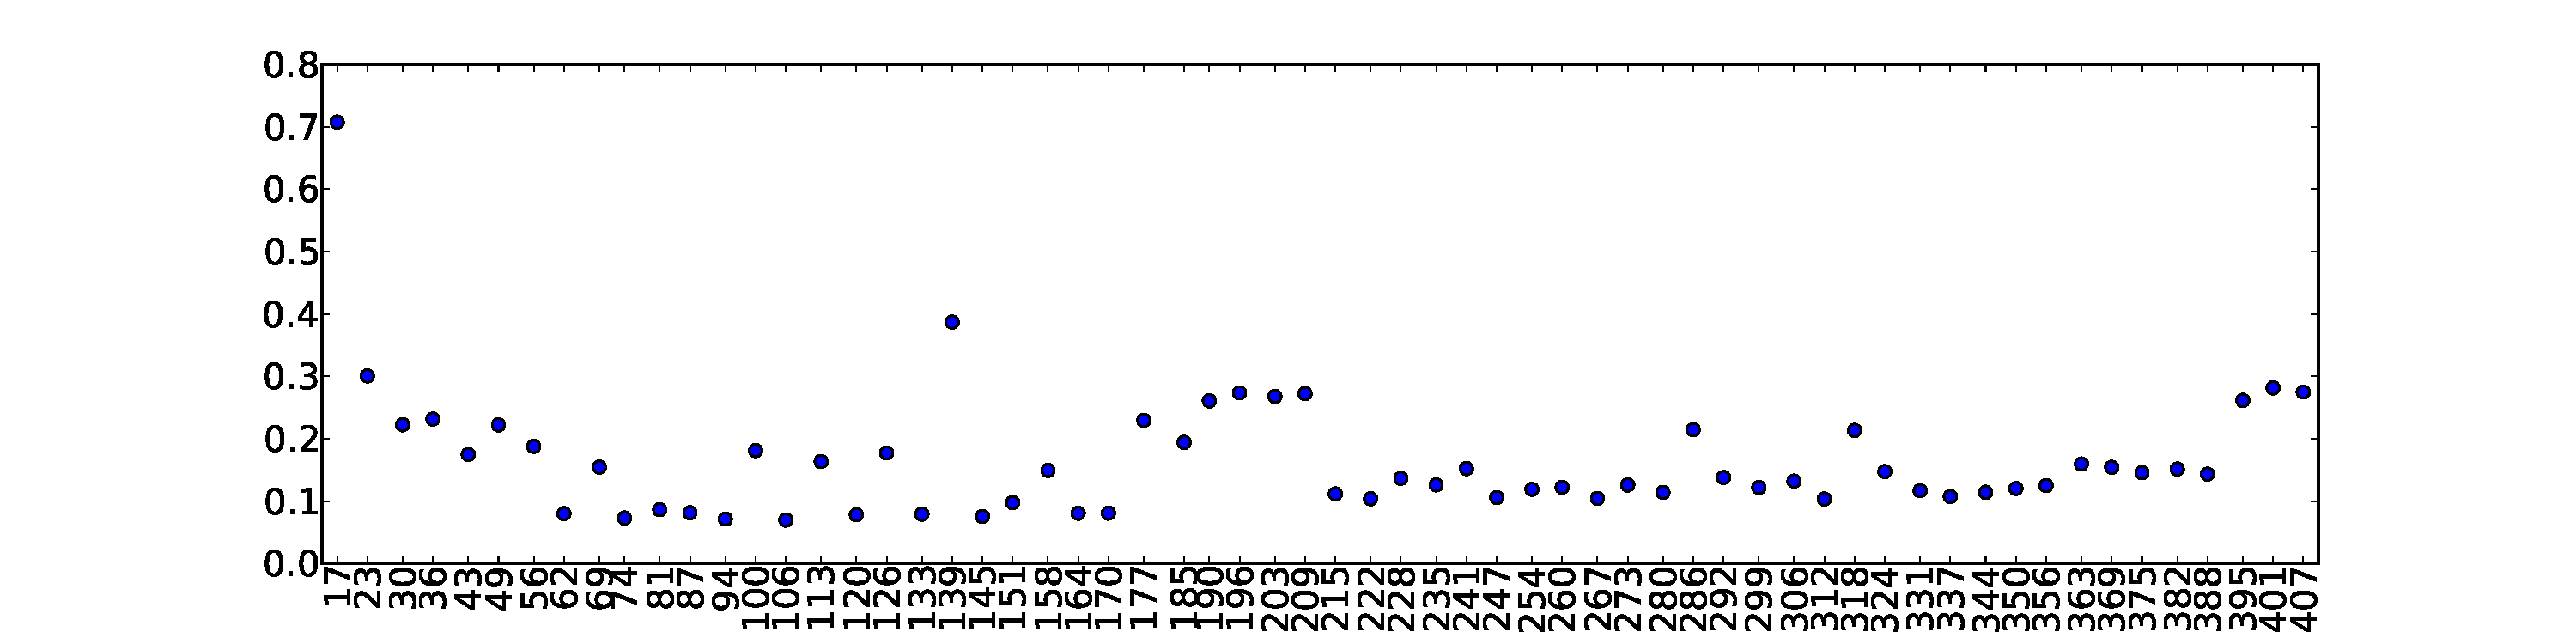
\includegraphics[height=2.5in,width=5.5in]{err_res_2_3_4_pointXX_cont.pdf}
	\caption{$\sigma_{\langle res\_2\_3\_4 \rangle}$ vs bar length}
	\label{fig5}
\end{figure*}

Fig. 6 shows the $\langle res\_2\_3\_4 \rangle$, but after re-analysis and comparing all the different fit methods. Note, the effect of the bin-width on the CSQ-WW method fits. Also keep in mind, there are some caveats to this plot, all for CSQ data points, for sometimes the fits failed or returned very biased resolutions (which is to be expected for now N and especially when bin-width=0.25) and those points were removed from the analysis. The point of this plot is to mainly show that the ``Flucations'' are not statistical and to additionally note the reason for using CSQWW in stead of CSQ and MLE.

\begin{figure*}[ht]
	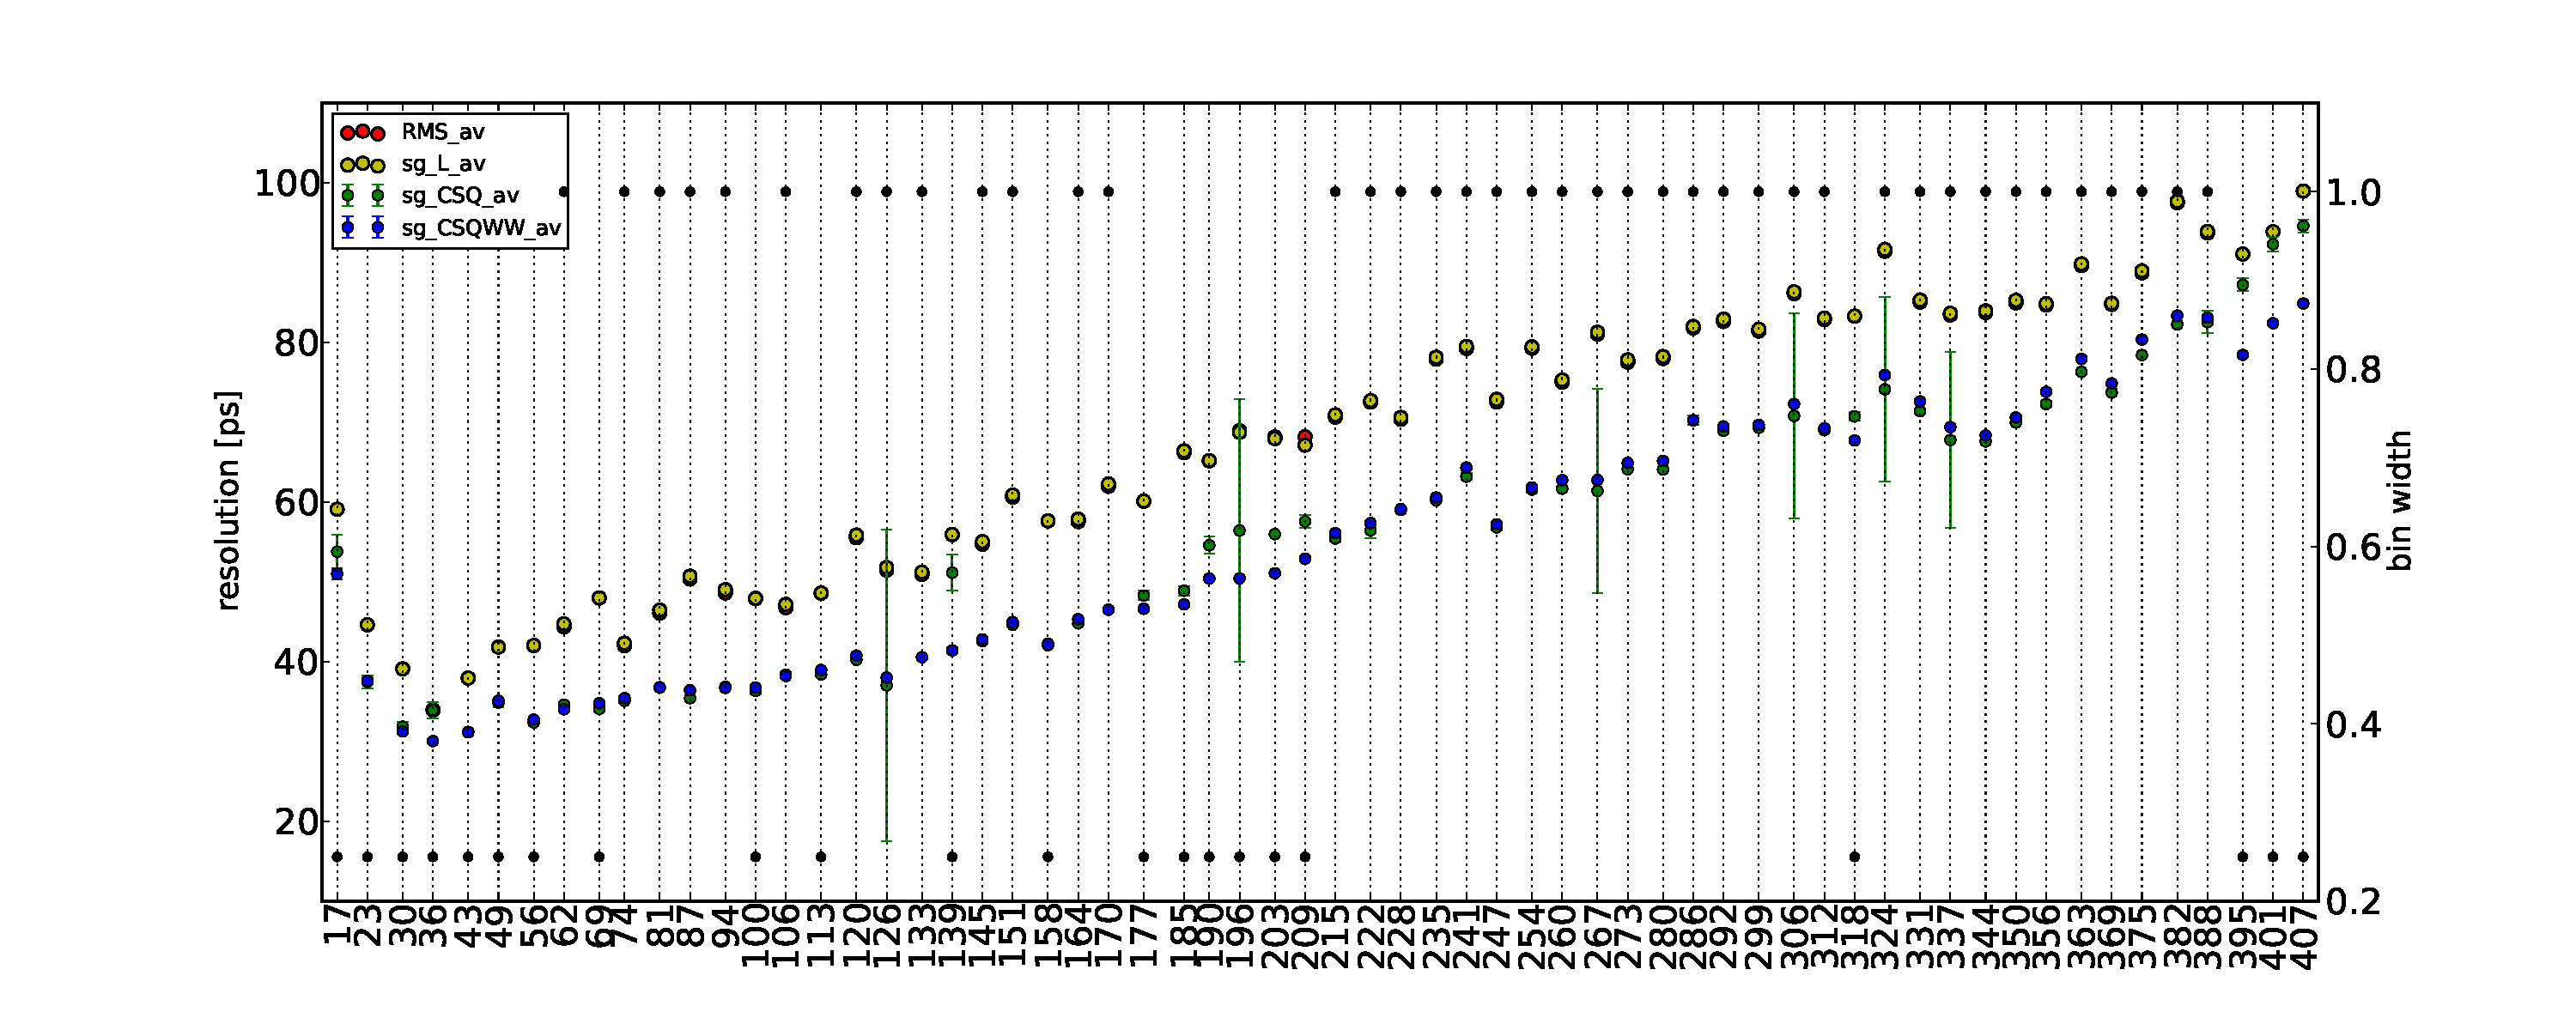
\includegraphics[height=4in,width=6in]{bar_stats_averages.pdf}
	\caption{ $\langle res\_2\_3\_4 \rangle$ re-analyzed using all fitting techniques}
	\label{fig6}
\end{figure*}

\clearpage

\section {Making sense of the ``Fluctuations'' in the propaganda plot}
The systematic (may need to be approximated for longer bars) and statistical errors need to be propagated when calculating single-bar resolutions since with more realistic errors bars, the plot may have a differnet quality to it. And then, perhaps, the correlation between $\langle single-bar-res \rangle$ and $\langle attenuation -length \rangle$ (see Fig. 7) will be more meaningful since the fact that the individual bar resolution does not correlate with the individual attenuation length (see Fig. 8) may not be a concern anymore if the error bars on the individual bar resolution is large.

\begin{figure*}[ht]
	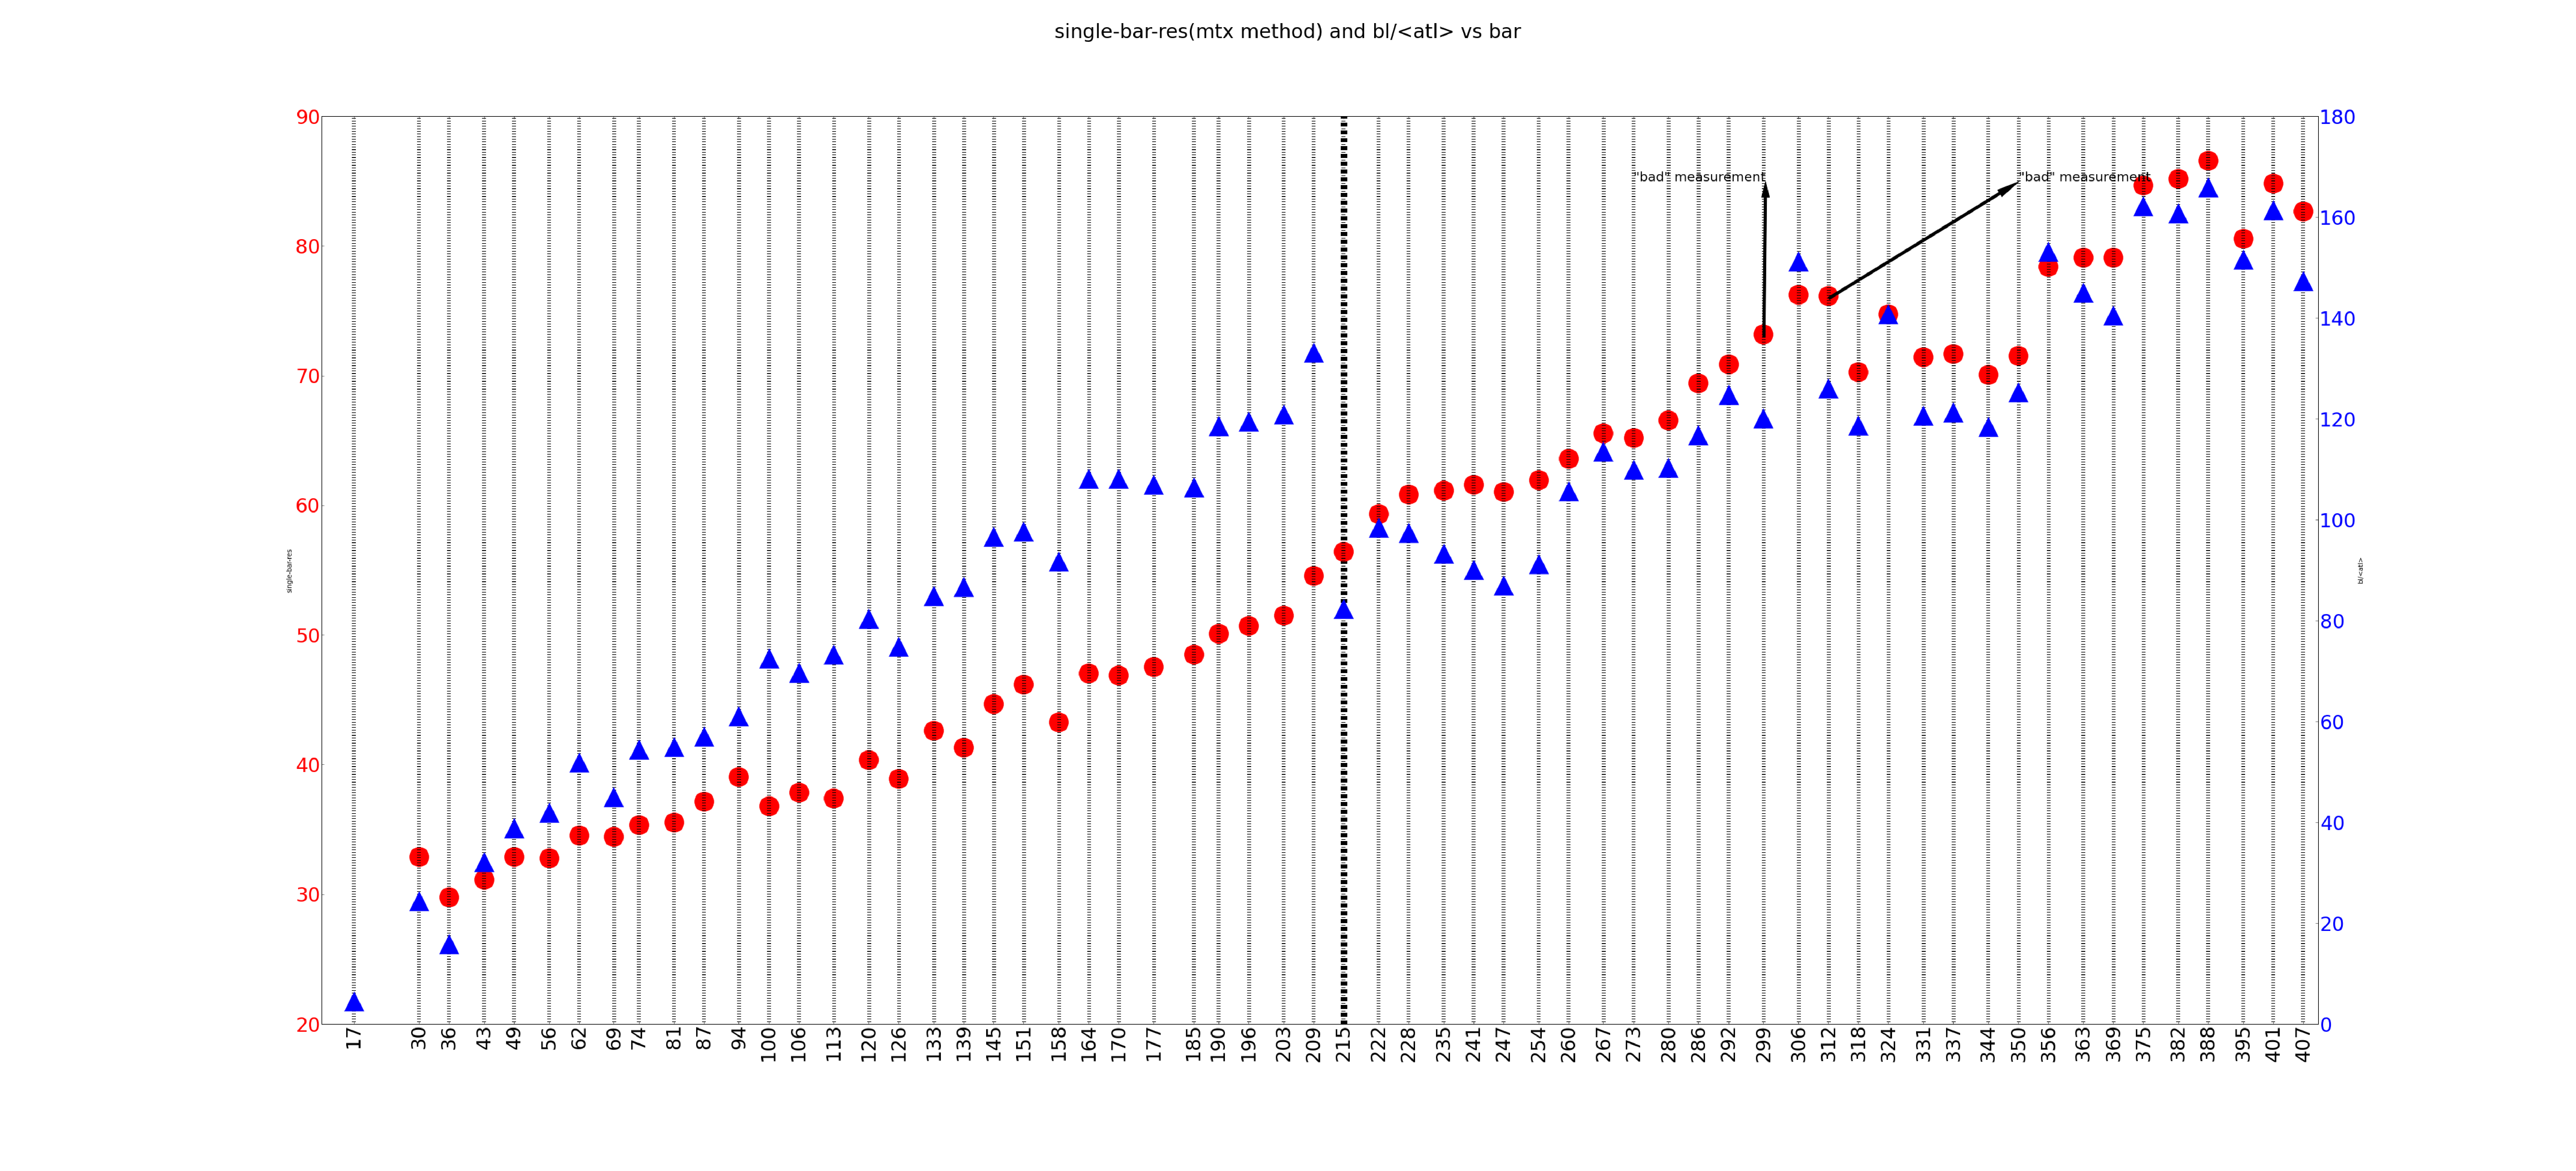
\includegraphics[height=3in,width=5in]{avg-res_avg-atl_vs_length-2.pdf}
	\caption{$\langle \text{single-bar-res} \rangle$ and  $\frac{\text{bar-length}}{\langle \text{attenuation-length} \rangle}$ vs bar}
	\label{fig7}
\end{figure*}

\begin{figure*}[ht]
	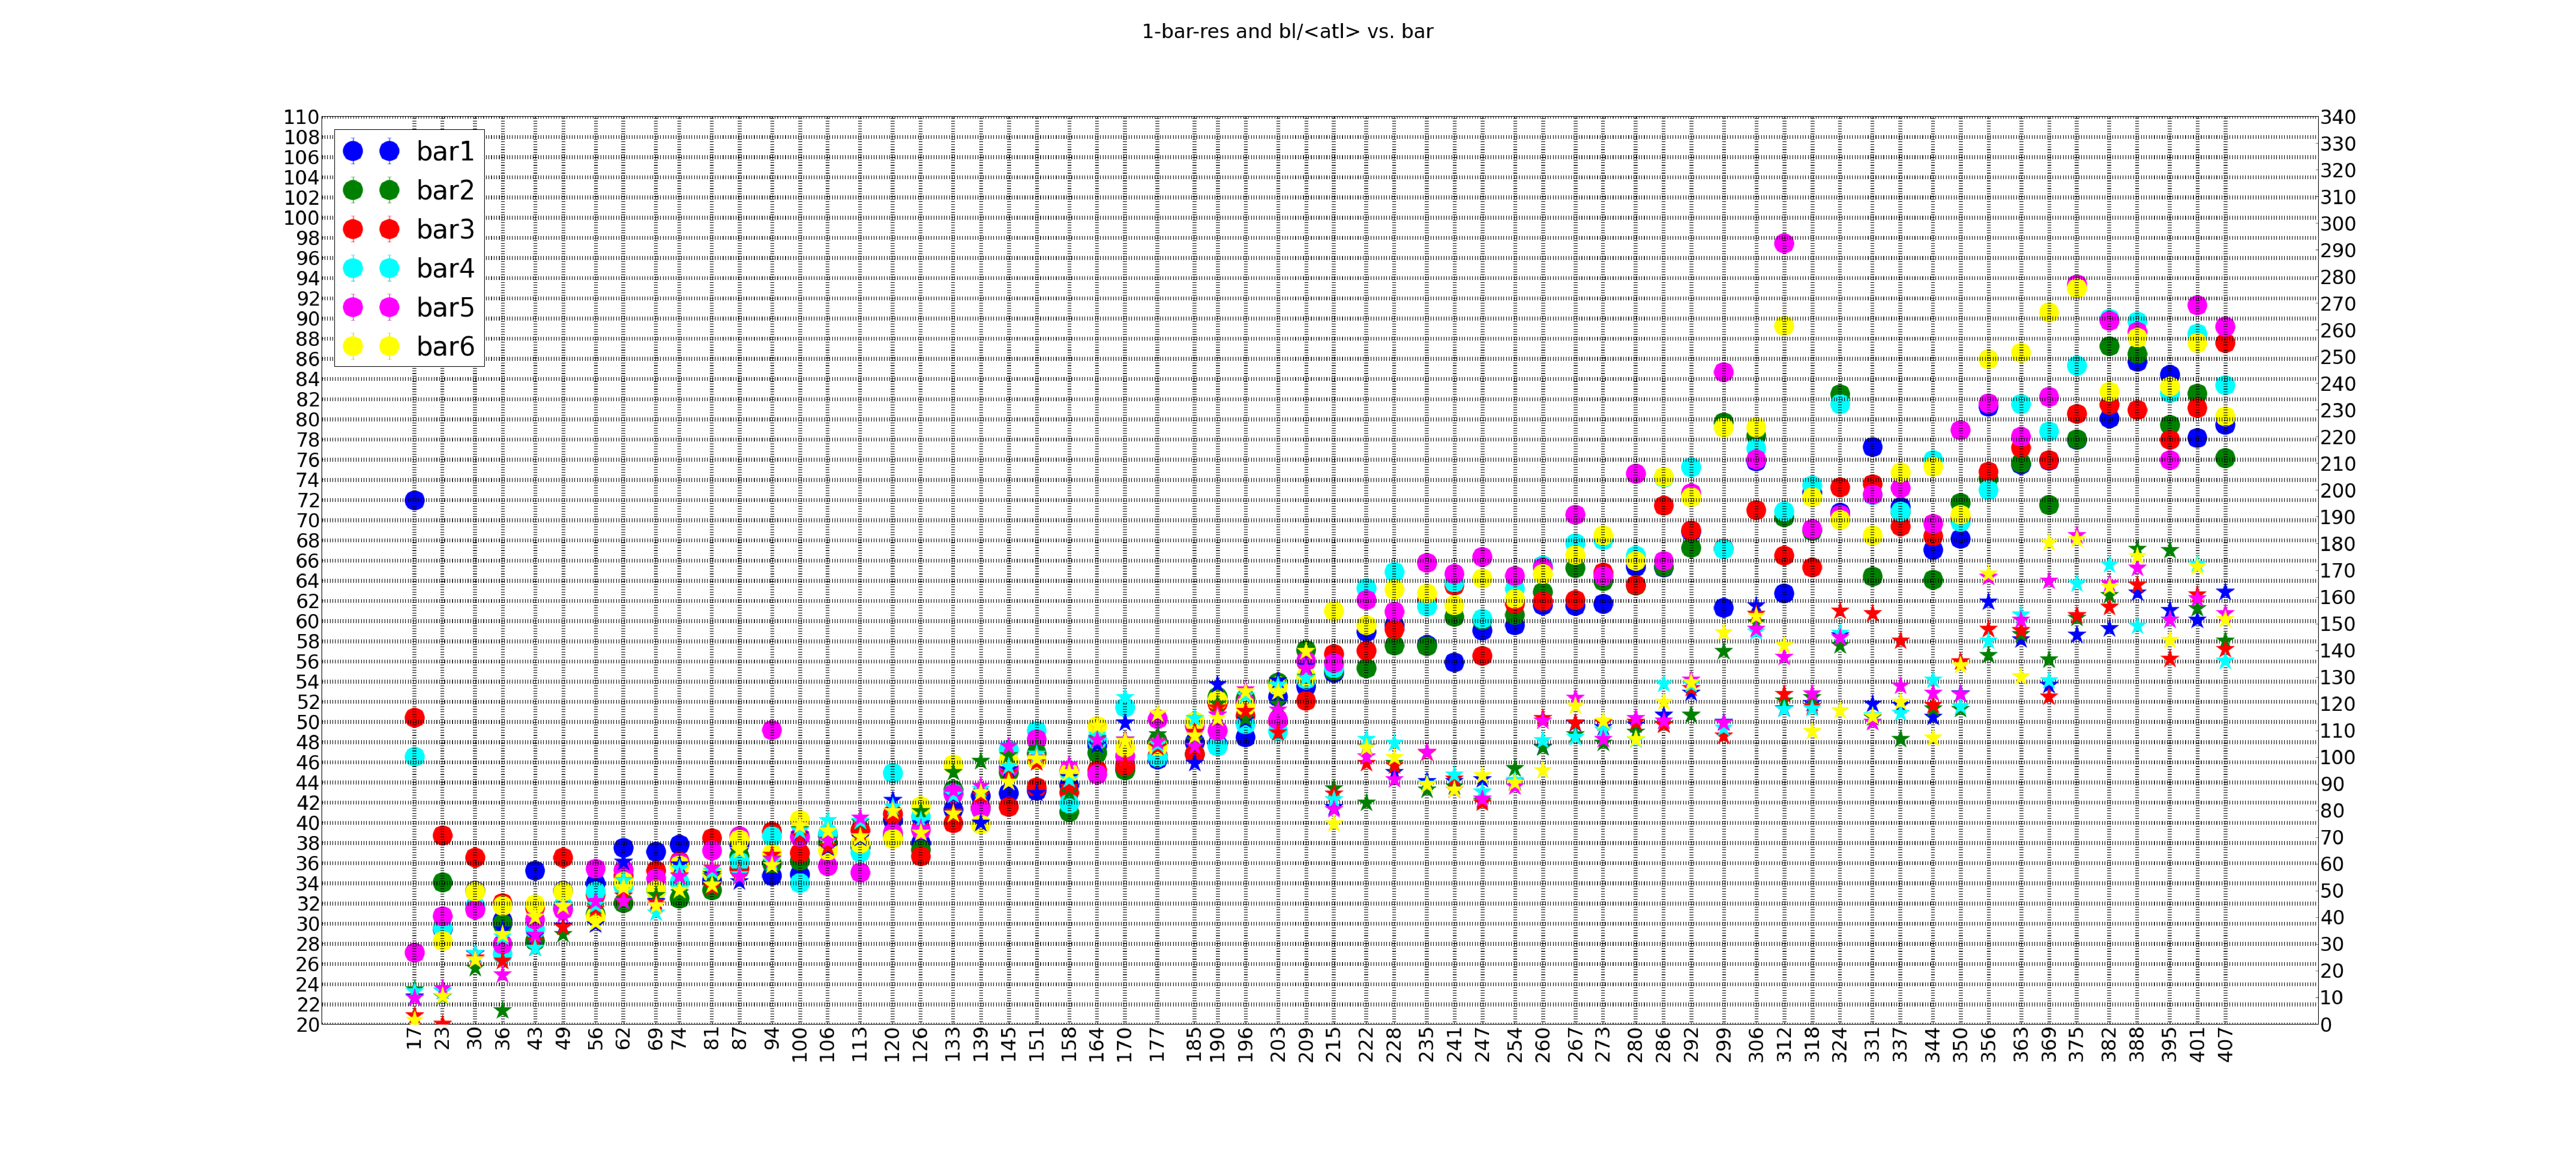
\includegraphics[height=4in,width=6in]{att-length-2.pdf}
	\caption{individual-bar-res individual-attenuation-length vs bar}
	\label{fig8}
\end{figure*}













% \phantomsection
% \addcontentsline{toc}{chapter}{Bibliography}
\label{bib}
\bibliographystyle{abbrv}
\bibliography{at_contrib}

\end{document}